\documentclass{article}
\usepackage[english]{babel}
\usepackage{booktabs} 
\usepackage[letterpaper,top=2cm,bottom=2cm,left=3cm,right=3cm,marginparwidth=1.75cm]{geometry}
 
\usepackage{amsmath}
\usepackage{graphicx}
\usepackage{subfigure}
\usepackage[colorlinks=true, allcolors=blue]{hyperref}
\usepackage[linesnumbered, ruled]{algorithm2e}
\usepackage{rotfloat}
%----------------------------------------------
\newcommand{\nomunit}[1]{%
\renewcommand{\nomentryend}{\hspace*{\fill}#1}}
\DeclareMathOperator{\erf}{erf}
%----------------------------------------------
\SetKwRepeat{Do}{do}{while}%

\title{
	\textbf{
      Accelerating Molecular Dynamics Simulations by FPGA with High-Bandwidth Memory (HBM2) Design
    }} 
\author{1,1,1,1,1,1}
\date{2024/10/23}

\begin{document}
\maketitle

%
% abstract
%
\begin{abstract}

\noindent
Molecular dynamics (MD) simulation is a powerful tool that models the behavior of particles over a given time interval, complementing biological and chemical experimental methods, particularly in materials science and drug discovery.
The speed of MD simulations is one of the key challenges that prevent their applications. 
To address this, a full hardware module based on field programmable gate arrays (FPGAs) has been designed to accelerate all parts of MD simulations. 
The solution aims to increase computational speed by utilizing pipeline techniques (Pipeline) to optimize the allocation of individual tasks within the entire parallel system.
We have also explored the impact of high-bandwidth memory (HBM2) on computational performance, comparing it with existing memory structures.
The work includes the use of DDR4 high-speed interfaces and the implementation of polling algorithms to improve access efficiency.
The optimized design of the underlying register-transfer level (RTL) circuitry for a single node has fundamentally enhanced the efficiency of data read and write operations to and from registers, with external storage read and write efficiency improved by more than 2.0 times.
The implementation of our work was demonstrated by comparing the simulation results of noble gas argon and dihydrofolate reductase (DHFR) with those obtained from OpenMM.
Additionally, potential strategies for continuing to improve the efficiency of MD simulations are also discussed.

\end{abstract}

\section{Introduction}

\noindent
MD simulations have shown critical importance in material and drug discovery due to its ability to provide detailed mechanistic insights into various material functions and biophysical interactions~\cite{fep_runtong,fep_york,md_in_dd_jmc2016,md_in_material1}. 
However, functionally-relevant processes are driven by the collective motions of molecules, most of which feature large spatial scales and long timescales that are computationally intensive to be model atomically by MD.
Contemporary mainstream MD implementations have incorporated multi-CPUs parallel strategies and GPU-based codes, aiming to extend the simulations scales accessible to modern computational power. ~\cite{charmm_at_c45,amber_gpu1,amber_gpu2,namd_gpu,omm7,gmx,2019arXiv190505359Y}.
Running MD simulations on supercomputers often takes a lot of time. The calculations of a large simulation system can take months to complete. Although most supercomputers are equipped with high-end parallel computing technology, they still need more powerful computing power for large-scale, long-term simulation tasks. To speed up the simulation and ensure accuracy, we delve into classical MD algorithms. Based on Amdahl's law, accelerated MD algorithms focus on two core problems: the calculation of non-bonding forces and the design of motion integrators. Conventional commercial software subdivides the calculation of non-bonding forces into Range Limited forces and Long Range forces~\cite{charmm_at_c45}. The finite range force includes van der Waals force calculation and the direct calculation part of PME calculation. The long range force is used to realize the PME inverse space calculation.\\

\noindent
In addition to GPU and CPU-based approaches, several research groups have reported the developments of novel hardware architectures dedicated to accelerate MD simulations. 
The commercial ANTON-series supercomputers utilized the Application Specific Integrated Circuit (ASIC) process and have up to 512 nodes of dedicated clusters~\cite{anton1,anton2,anton3}.
However, the ANTON series of supercomputers are expensive to design, have long commissioning and development cycles, and can not easily access. 
Additionally, the MD-GRAPE series, which dates back to the late 1980s, uses Microcontrollers (MCUs), Complex Programmable Logic Devices (CPLDs), Field Programmable Gate Arrays(FPGAs), and other acceleration circuits to build a multi-node design~\cite{MD-GRAPE-3,MDGRAPE-4A}.
This design is combined with a specialized fiber-optic transmission network to form a large-scale computational cluster. 
The MD-GRAPE series has been developed through four generations, and its hardware devices are constantly updated and iterated, but the design cost remains very high. 
Furthermore, the Novo-G series, which uses commercial FPGA accelerator cards from the Intel series, optimizes MD computational efficiency from both hardware and software perspectives~\cite{Novo-G,Novo-G2,3dfft,bondforce}.\\
% add comment for the Novo-G

\noindent
Although FPGAs are less dense and slower than ASICs, they offer greater design flexibility, are more cost-effective, and consume less power compared to other devices \cite{ref3}. 
FPGAs incorporate a variety of unique production techniques, such as the FLASH process and the reverse fusion process, which allow them to support multiple reconfigurations and debugs in the commercial sector, accommodating different experimental design needs \cite{ref22}. 
In the chip design phase, FPGA design is considered the core of prototyping, indicating that FPGA circuit design has significant potential for practical application in the later stages of conversion into an ASIC process \cite{ref3,ref18}. 
Therefore, using FPGAs to accelerate MD simulations remains a promising approach.\\

\noindent
Motivated by the desire to accelerate MD simulations, a full hardware module has been designed to speed up all aspects of the MD computation. 
This module aims to increase computational speed and utilizes pipeline techniques to optimize the allocation of tasks in the entire parallel system \cite{ref12,ref23}. 
Additionally, we have built a software framework dedicated to SIMD (Single Instruction, Multiple Data) to enhance the data processing capabilities of the circuit. 
Our work is structured as follows: in Section 2, we revisit the critical algorithms in MD simulations and discuss our considerations for improving their performance. 
In Section 3, we present the architecture implemented in this work, followed by comparison results that highlight the necessity of our approach. 
Finally, we demonstrate the results of MD simulations of argon and DHFR using our implementation and compare them with results obtained from OpenMM to validate the correctness of our approach.
\\



\section{Basic algorithms of classical MD and force field}

\noindent
In this work, we divide a classical MD program into four parts~\cite{ref1}:
\begin{enumerate}
\item Read in the specified simulation conditions, such as initial temperature, particle number, and time step.
\item Determine the initial positions and velocities of the particles.
\item Compute the forces acting on the particles.
\item integrat Newton's equations to update velocities, and positions of all particles.
\end{enumerate}
Repeat steps 3 and 4 until the user specified simulation step is met. 
In classical MD simulations, the force acting on each atom is often calculated using force fields which will be discuss in the next two subsection.
Then integration of Newton's equations over the time step is achieved by algorithms named integrator which is discuss in the 3rd subsection.


\subsection{Bonded force}

\noindent
Most force fields model interactions between particles using bonded and nonbonded terms:
\begin{equation}
    \boldsymbol{F}^{\text {total}} = \boldsymbol{F}^{\text {bonded}} 
                                    + \boldsymbol{F}^{\text{non-bonded}}
\end{equation}
,where the bonded force consists of bond, angle, dihedral and improper terms:
\begin{equation}
\boldsymbol{F}^{\text {bonded}} = \boldsymbol{F}^{\text {bonds}} 
                                    + \boldsymbol{F}^{\text {angles}} 
                                    + \boldsymbol{F}^{\text {dihedrals}} 
                                    + \boldsymbol{F}^{\text{impropers}}
\end{equation}

\noindent
Most bonded terms are modeled by harmornic potentials, except the dihedrals are modeled using a summation of cosine functions.
Because the bonded terms are only calculated when bonds exists between atoms, their computational cost can be regards as $\mathcal{O}(N)$.\\


\subsection{Nonbonded force}

\noindent
The non-bonded terms often consist of van der Waals (vdW) and Coulomb terms:
\begin{equation}
    \boldsymbol{F}_{i,LJ}\
    =\sum_{j \neq i} \frac{\epsilon_{a b}}{\sigma_{a b}^{2}}\left\{12\left(\frac{\sigma_{a b}}{\left|\mathbf{r}_{j i}\right|}\right)^{14}-6\left(\frac{\sigma_{a b}}{\left|\mathbf{r}_{j i}\right|}\right)^{8}\right\} \mathbf{r}_{j i}
\end{equation}
    
\begin{equation}
    \boldsymbol{F}_{i,Coulomb}=
        \frac{q_{i}}{4 \pi \epsilon} \sum_{j \neq i}  
        \left\{\frac{1}{\left|\mathbf{r}_{j i}\right|}\right\}^{3}  
        \mathbf{r}_{ji}
        \label{eqn:coulomb}
\end{equation}
where, the $\epsilon_{a b}$ and $\sigma_{a b}$ are parameters of particles.
Because the non-bonded force need to be calculated between nearly all pair-wise particles, the computational cost is $\mathcal{O}(N^2)$.
Thus the bottom neck in MD is the calculation of nonbonded terms.

\noindent
Because the decay of coulomb force is slow with distance. it is always calculated with the particle mesh Ewald PME algorithm in a perodical system to handle the long-range Coulomb forces. 
Assuming that the unit cell is square, the Coulomb potential on atom $i$ can be expressed as Eq~\ref{eqn:coulomb}. 
The algorithm utilizes spherical Gaussian positive and negative charges with the same distribution to partition $E^\mathrm{Coulomb}_i$ into real and inverse parts. 
The real part converges fast in real space and is safe to truncate at the cutoff, and the inverse part is also fast converging, but in in the inverse space.
The electrostatic potential energy of the simulated system under PBC is expressed as:


\begin{center}
	\begin{equation}
		E_{Coulomb}=\frac{1}{4\varepsilon \pi} \cdot 1/2 \sum_{n}^{} \sum_{i=1}^{N} \sum_{j=1}^{N} \frac{q_{i}q_{j} }{\left|r_{ij}+nL\right|} 
	\end{equation}
\end{center}
The simulation box is a square of length $L$, where the number of charged particles is $N$. $r_{ij}$ is the distance between particle $i$ and particle $j$, and $\epsilon$ is the vacuum dielectric constant. 
The simulation lattice extends indefinitely in the control according to the periodic boundary conditions, and $n$ is an integer.

\begin{center}
	\begin{equation}
		E =E_\mathrm{dir} +E_\mathrm{rec}+E_\mathrm{corr}
	\end{equation}
\end{center}

\noindent
The Gaussian distribution function is introduced into the Ewald summation algorithm and consists of three parts after being processed by the PME algorithm:

\begin{center}
	\begin{equation}
		E_\mathrm{dir} = \frac{1}{2} \sum_{n} \sum_{i,j=1}^{N} \frac{q_i q_j \erf{\left( \beta\left|\mathbf{r}_j - \mathbf{r}_i+\mathbf{n}\right|\right)}}{\left|\mathbf{r}_j - \mathbf{r}_i + \mathbf{n}\right|}
	\end{equation}
\end{center}

\begin{center}
	\begin{equation}
		E_\mathrm{rec} = \frac{1}{2\pi V}\sum_{m\neq0}{\frac{\exp{\left( -\pi^2\mathbf{m}^2/\beta^2 \right)}}{\mathbf{m}^2}S\left( \mathbf{m} \right) S \left( -\mathbf{m} \right)}
	\end{equation}
\end{center}

\begin{center}
	\begin{equation}
		E_\mathrm{corr}=-\frac{1}{2}\sum_{\left( i,j \right)\in M}\frac{q_i q_j \erf{\left( \beta\left|\mathbf{r}_i-\mathbf{r}_j\right| \right)}}{\left|\mathbf{r}_i-\mathbf{r}_j\right|}-\frac{\beta}{\sqrt\pi}\sum_{i=1}^{N}q_i^2
	\end{equation}
\end{center}
,where the $\beta$ is called Ewald's coefficient, which regulates the speed of convergence of real space and Fourier space. 
The larger its value, the faster the real space converges and the slower the Fourier space converges and vice versa.
The $\erf$ is the Gaussian error function.\\


\noindent
To improve computational efficiency, the finite-range force in the direct space uses a proximity list lookup method. 
This method obtains the spatial relationships between particles using their coordinates and distances, and stores this data in a neighborhood list. 
When affected by short-range forces, a particle only interacts with its neighboring particles. 
As the distance increases, all particles in the neighborhood are treated as neighbors, and their coordinates are updated to reconstruct interrelationships in a new step. 
The neighbor list is constructed based on each particle's position within a specific region, assuming that the interaction force between particles is truncated at a radius $r_cut$.Each particle contains a list of potential neighboring particles, which serves as input for the next computational cell.
In addition, for periodical system, each simulation cell has 26 adjacent cells in the whole space. 
According to Newton's third law, to reduce repeated calculations, only the particle pairs in the 13 neighboring cells in the upper half of the center cell are filtered and calculated.\\



\subsection{Verlet integrator algorithm}

\noindent
Given the force acting on each particle, the velocity and position is updated by integrator. 
Commonly used integrators include the Verlet algorithm and its variants, such as the Velocity Verlet and Leap-frog methods. 
Using the acceleration and position at time $t_0$, the position ($\mathbf{r}$) and velocity ($\mathbf{v}$) of next step are obtained:

\begin{equation}
    \mathbf{r}_{i}(t_{0}+\Delta t ) = 
        2\mathbf{r}_{i}(t_{0}) - \mathbf{r}_{i}(t_{0}-\Delta t) + (\Delta t^2/m_{i}) \boldsymbol{F}_{i}(t_{0})
\end{equation}

\begin{equation}
    \mathbf{v}_{i}(t_{0}) = 
        (\mathbf{r}_{i}(t_{0}+\Delta t )-\mathbf{r}_{i}(t_{0}-\Delta t ))/2\Delta t
\end{equation}

\noindent
The Verlet algorithm requires a motion update calculation for each particle ($i$) in thesystem, and the calculation requires a two-step difference formulation. 
It needs to utilize the position information of the particle at the previous moment $\mathbf{r}_{i}(t_{0}-\Delta t)$ and the acceleration $\boldsymbol{F}_{i}(t_{0})/m_{i}$ and position information at the current moment $\mathbf{r}_{i}(t_{0})$ . 
In implementing the algorithm, the position and acceleration of the current moment and the position of the previous moment need to be stored.\\


\begin{figure*}[ht]
\centering
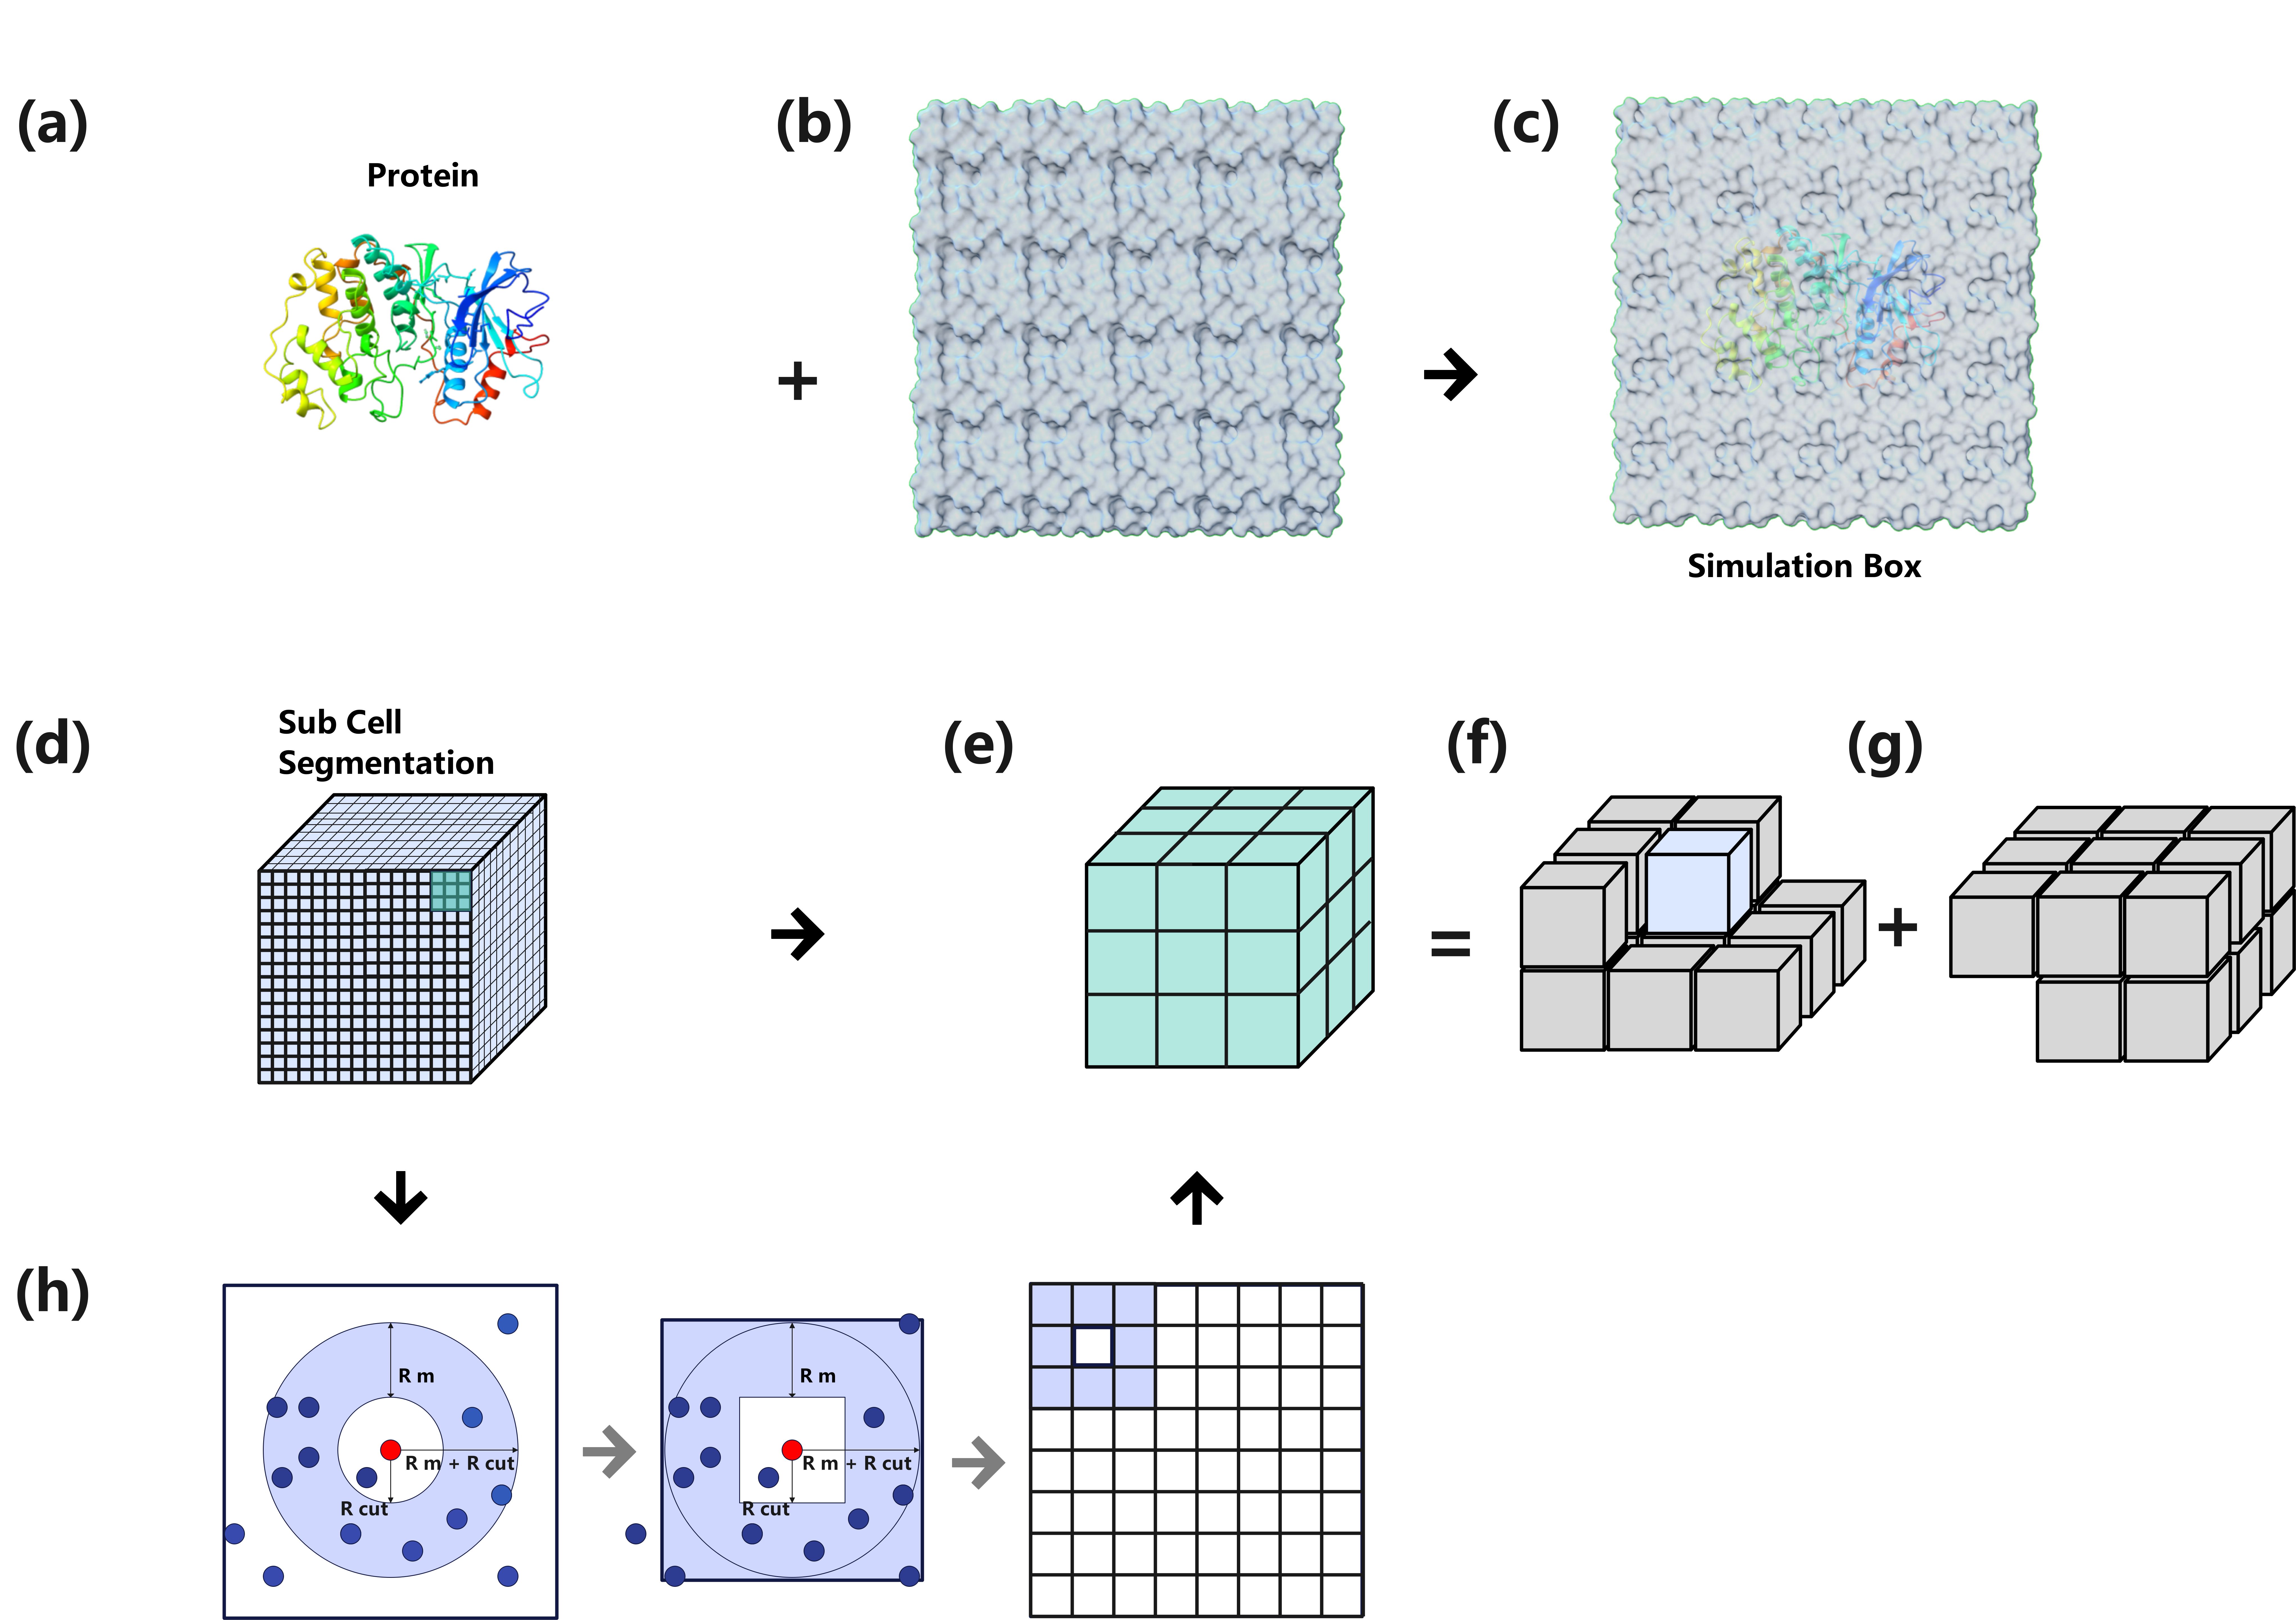
\includegraphics[angle=0,width=1.0\textwidth]{./figures/Fig1_Neighboursegment.png}
\caption{ The protein structure of DHFR(a) and cuboid simulated water box (c) were cut into Cells of equal size by Verlet algorithm (d).
	Among them, Home Cell and the surrounding 26 Neighbor cells (e), of which the upper and lower two are divided into "upper hemisphere"(f) and "lower hemisphere"(g).
	(h)According to the Verlet algorithm, the center particle and the surrounding particles can be divided into equal-sized squares according to the values of $Rm$ parameter and $Rcut$ off}
\end{figure*}



% the 3rd section
\section{Proposed architecture}

\begin{figure*}[ht]
	\centering
	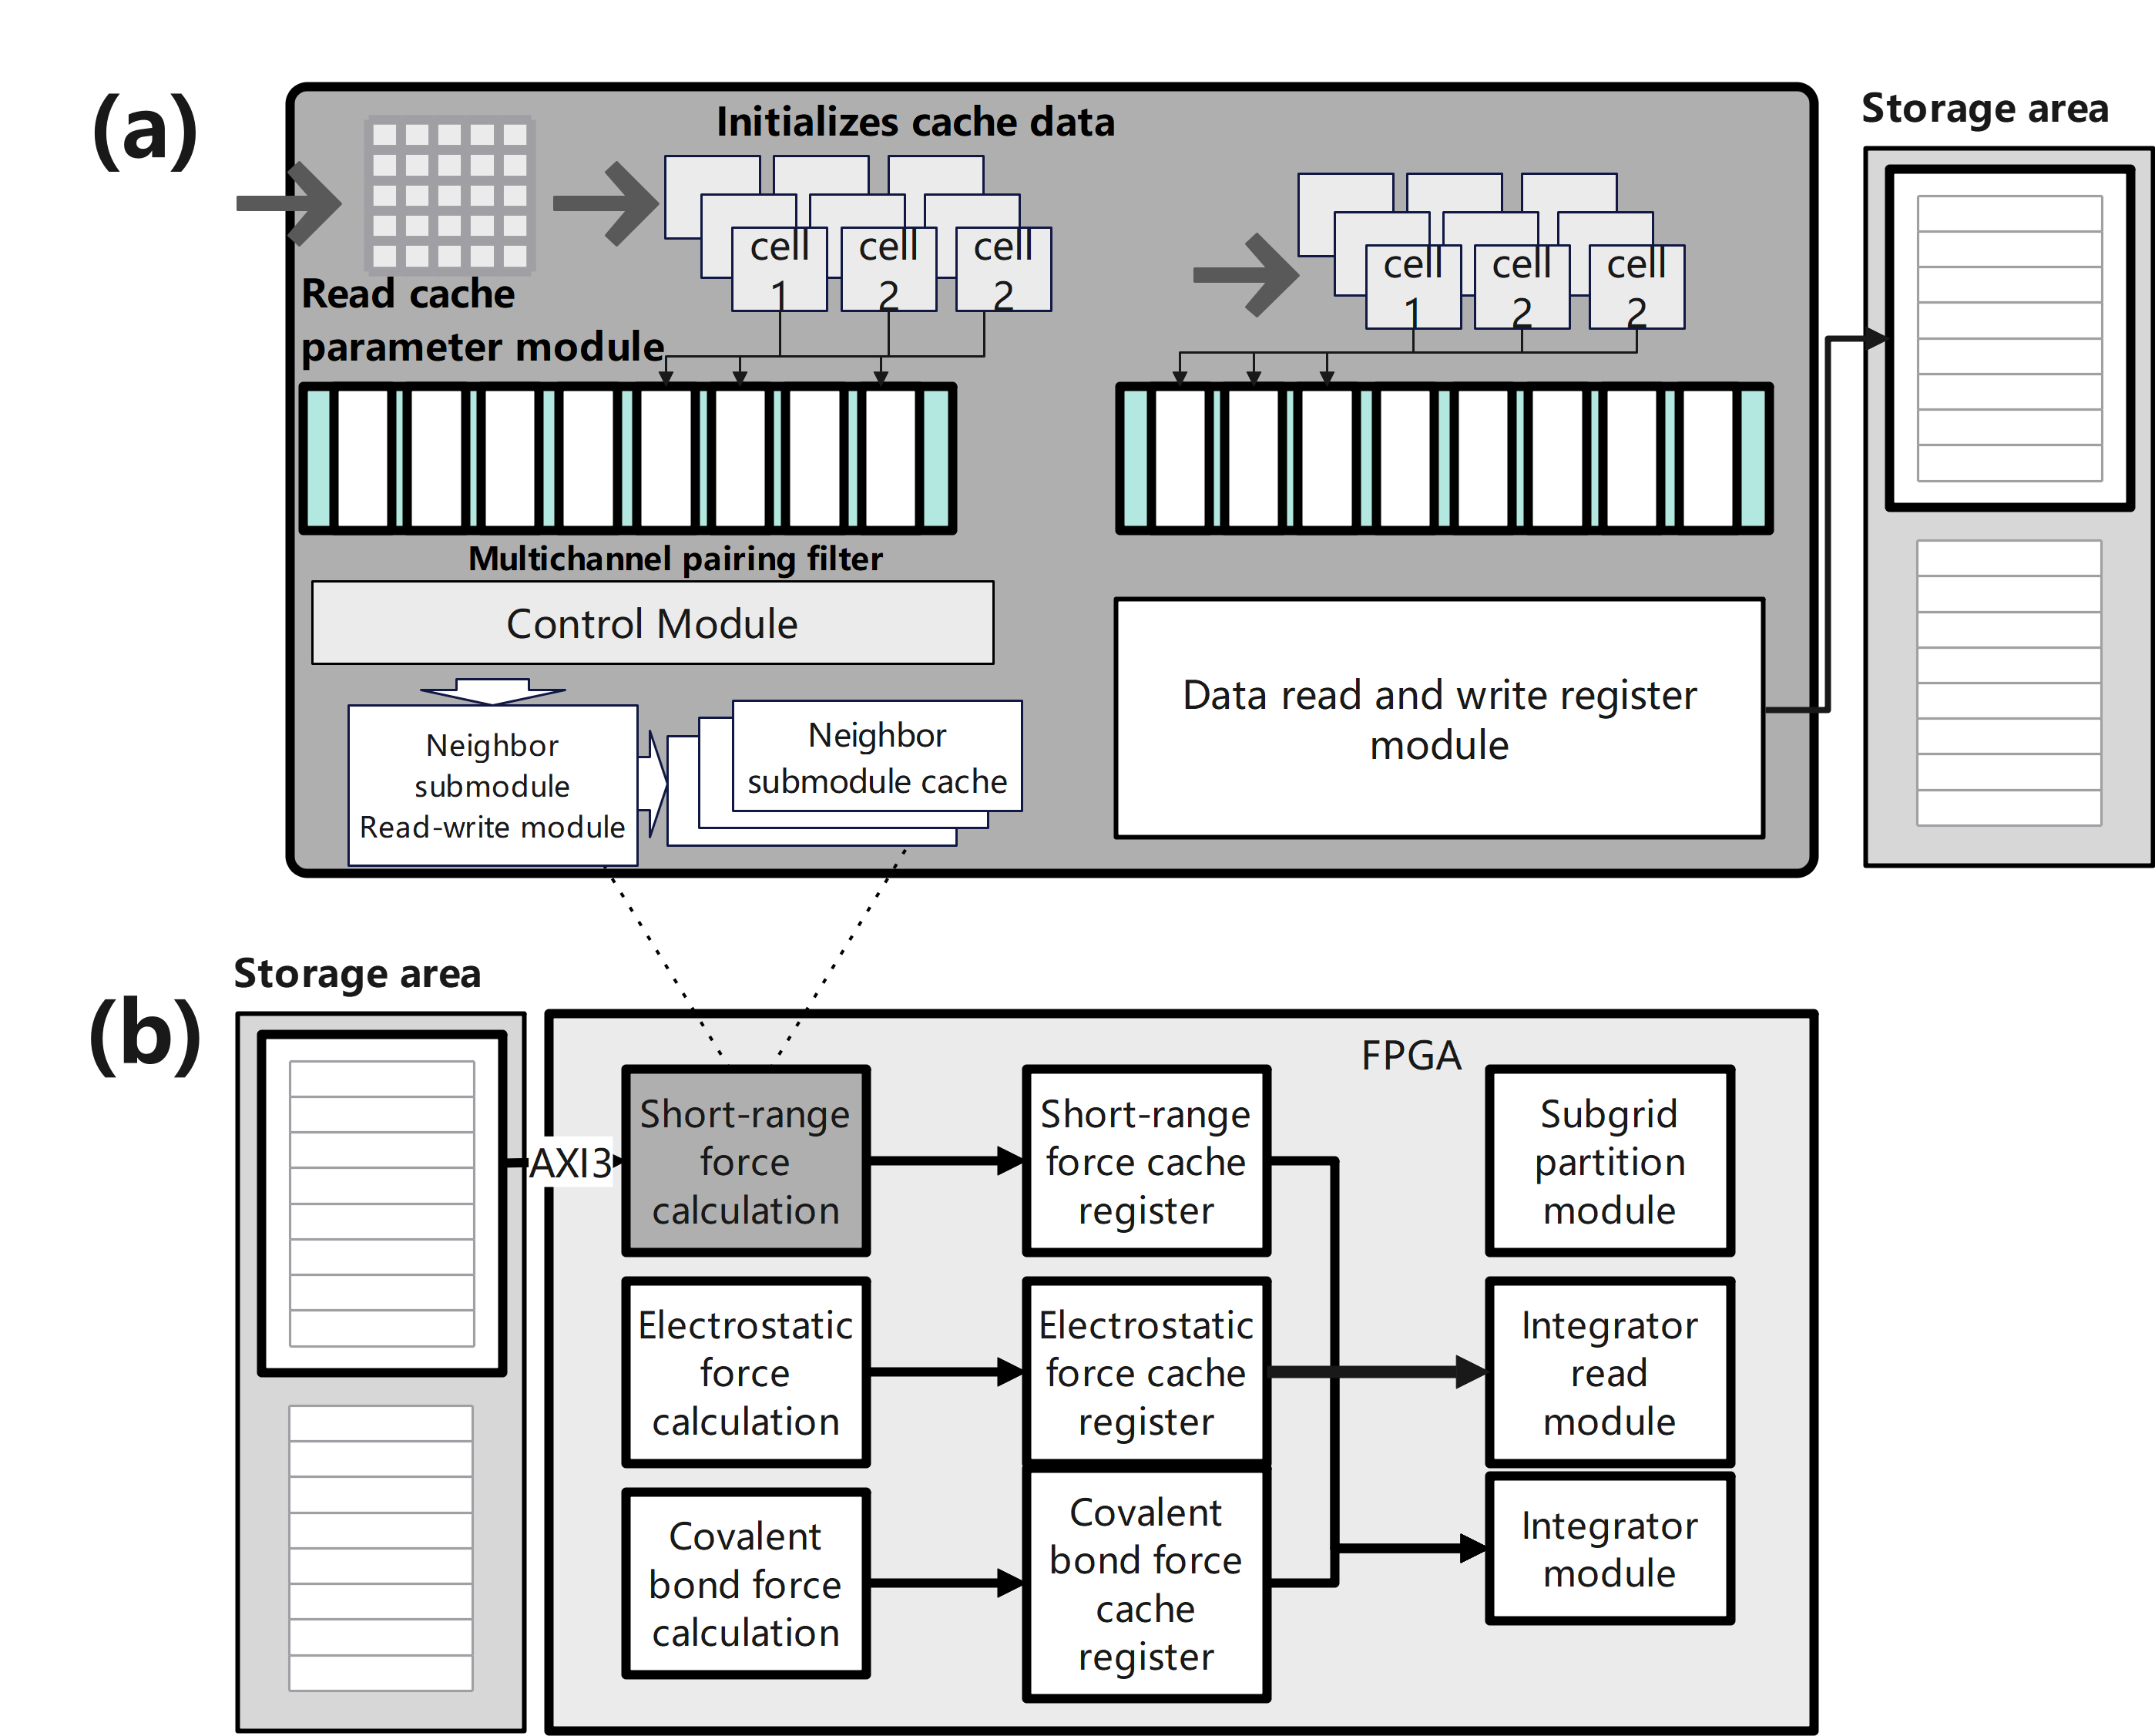
\includegraphics[angle=0,width=1.0\textwidth]{./figures/Fig2_top_module_a_b.png}
	\caption{Block diagram of the implementation of the finite range force calculation module. Module b, for a single FPGA acceleration card, the user logic resources MD hardware computation is mainly divided into short-range force force, long-range force force and covalent bonding force three kinds of processing units. Module a,The whole RL module is composed in each sub-module of the frame.}
	\label{fgr:implementation}
\end{figure*}


\noindent
Based on MD algorithms, we proposed a design to accelerate MD simulations on 
FPGA. 
As shown in Figure~\ref{fgr:implementation}, the data processing flow in the RL 
module is as follows:
The CPU preprocesses MD simulation data, assigning each particle to a unique 
cell based on the cell serial number obtained by segmenting the original data.
Particle information is then bound to the cell serial number. 
The side length of each cell is determined by the truncation distance, and the 
number of cells is determined by the simulation dataset's rectangular space. 
Each cell contains information about its particles and neighboring cells, 
forming a data table stored in memory.\\

\noindent
Each particle occupies one row of storage space. 
The starting position of each data cell is directly located using the cell 
serial number while the data cell length is determined based on the maximum 
number of particles with an appropriate margin. 
% 这里什么意思？
The exclusion information data table, containing information from bonded 
particle pairs, is stored in memory.
The structure of the data table excludes particle information in pairs and the 
number of excluded particles as well as their storage addresses are configured 
in registers for use by relevant modules. 
The proximity force calculation uses interpolation and coefficient tables, 
which are prepared by the CPU and configured in the FPGA's RAM. 
After configuration, the CPU starts the prefetching particle data unit to 
execute the next operatio and the paralleled particle 
reading module provides the particle pair information for calculation.\\

\noindent
Next, the multi-channel calculation filter module processes each data cell as 
the main cell. 
It retrieves particle information from the main cell and the first 13 related 
cells, forming particle pairs for distance calculation. 
Each particle from the main cell is paired with one particle from each of the 
13 neighboring cells, and the distance is calculated. 
The module then selects particle pairs have a distance within the cutoff for 
further calculation. 
% 能不能引用一下精简一下这段？
Interpolation table coefficients are obtained based on the squared distances of 
the selected particle pairs and the particle type information. 
These coefficients, based on charge information, are used for electrostatic and 
short-range force calculations. 
All parameters for the limited-range force calculation are stored in the FPGA's 
on-chip RAM and passed to the particle distance judgment module. 
Only particles within the distance range proceed to the next step in the force 
calculation pipeline. 
The calculation progress is monitored by the proximity force calculation 
module, which updates the force calculation result data table and supervises 
the progress.\\

\noindent
%过渡一下
The proximity force calculation unit contains several calculation pipelines to 
match the force requirements of upstream and downstream modules. 
The calculator performs all proximity force calculations and decomposes the 
results into 3D coordinates based on the finite-range forces of the 
particle pairs. 
The force from the same particle to different particles in each main cell is 
accumulated and cached and the force from the first 13 neighboring cells are 
cached in the particle pair force cache RAM according to the particle serial 
number. 
All force results and part of the accumulated force data are cached in the 
corresponding areas based on the particle number at the source end. 
At least two accumulator pipelines and two memory entry generation modules are 
reserved for parallel processing to match the upstream and downstream 
processing capabilities.\\



\subsection{Data is read and written using HBM memory.}
\noindent
The high-bandwidth memory (HBM) stores data cells with structured organization.
% 图几？
As illustrated in the accompanying diagram, each data cell configuration 
comprises multiple information layers.
The primary row specifies fundamental metadata including the cell serial 
number, physical dimensions, particle count, particle information offset 
addresses, and verification codes.
Subsequent quadrants systematically document adjacency relationships through 
serialized identifiers and HBM address offsets for neighboring cells, with each 
spatial dimension represented in consecutive 8-byte blocks. 
The memory allocation follows strict alignment protocols where incomplete rows 
are padded to achieve full row boundary compliance. 
Particle-specific serial numbers are sequentially stored in contiguous memory 
segments, maintaining the established alignment convention through terminal 
padding.
This hierarchical arrangement ensures efficient data retrieval while preserving 
memory architecture integrity.
%???
Data cached at the same address, multiple channels read simultaneously; Data 
cached at the different address, multiple channels read simultaneously shown in 
Figure~\ref{fig:subfig1}and Figure~\ref{fig:subfig2}.\\

\subsubsection{Particle information storage table Home Cell and Neighbor Cell 
storage relationship.}
\noindent
Data cells accommodate individual particles through dedicated row allocations, 
with their dimensional parameters determined during preprocessing by the 
maximum anticipated particle count augmented by a defined safety margin. 
A hierarchical addressing mechanism enables direct access to any data cell 
using its unique serial number, which maps to precise memory coordinates. 
Structural omission of paired particle entries generates the specialized memory 
topology detailed in associated documentation, with exclusion criteria governed 
by registers storing both the count and physical addresses of excluded 
elements-parameters directly utilized by downstream computational modules. 
Critical to force calculations, interpolation coefficients and lookup tables 
are precomputed by the CPU and loaded into dedicated on-chip RAM resources 
within the FPGA fabric. 
Exclusion data originates from predefined covalent bonds, where paired particle 
identifiers are aggregated into composite exclusion records stored natively in 
HBM arrays, ensuring low-latency access during simulation execution.\\

\subsubsection{The storage relationship between Home Cell and Neighbor Cell in 
the particle information storage table.}

\noindent
The particle information storage architecture establishes a dual-layer 
hierarchy between HomeCell and NeighborCell structures operating on 512-bit 
data buses, where non-functional regions undergo zero-padding optimization to 
maintain address alignment and facilitate efficient lookup operations as shown 
in Figure~\ref{fig:subfig3}(b). 
This unified storage schema integrates 7 distinct functional segments 
characterized by predefined bit allocations: initial addressing utilizes a 
lookup code for rapid data classification, directing processing pipelines to 
appropriate computational modules based on encoded metadata. 
Serial number assignment implements a globally unique addressing scheme across 
all simulation entities, while spatial coordinates embed precise 3D positioning 
parameters compliant with cartesian coordinate systems. 
Particle identifiers adopt globally unique numbering conventions to track 
individual entities throughout simulation lifecycles. 
The system employs a hybrid addressing paradigm where hierarchical indexing of 
cell relationships coexists with direct particle access patterns, supported by 
register-mapped exclusion tables that dynamically configure FPGA resources for 
force calculation acceleration. 
This structured approach enables deterministic memory access latencies while 
preserving compatibility with parallel processing architectures.\\

\subsubsection{The data structure of the particle information storage table 
Home Cell.}
\noindent
The particle information repository employs a fixed-length encoding scheme 
within 512-bit HomeCell structures, adhering to memory alignment constraints 
through zero-padding strategies that optimize address resolution efficiency 
(shown in Figure~\ref{fig:subfig3}(c)). 
This standardized format segments data into 5 predefined fields with dedicated 
bit allocations, initiating with a machine-readable type identifier that 
directs processing workflows to designated arithmetic units. 
Each particle's physical attributes—including scalar charge magnitudes, vector 
velocity components, and 3D Cartesian coordinates are encoded using IEEE 
754-compliant 32-bit floating-point representations for numerical stability.\\
% cite paper or document for IEEE 754 ^

\noindent
Parallel processing requirements necessitate dual-tier memory management: 
precomputed pairwise interaction data for the first 13 nearest NeighborCells 
resides in on-chip registers for immediate access, while remaining 13 required 
neighbor interactions are staged in 256-bit wide global memory buffers as shown 
in Figure~\ref{fig:subfig3}(c). 
This partitioning balances latency-critical intra-cell computations with 
bandwidth-intensive inter-cell calculations, facilitated by FPGA-optimized 
neighbor index register files that minimize off-chip memory transactions. 
The hybrid storage methodology simultaneously satisfies deterministic timing 
constraints for core physics kernels while maintaining scalable data handling 
capacity for large-scale particle systems.\\

\subsubsection{The Home Cell and the remaining 13 neighbor cells accumulate the 
results}
\noindent
The particle-to-force caching and partial summation module implements 
latency-optimized data reuse by sequentially capturing force calculation 
results between a primary cell's particle and its intra-cell counterparts 
across successive clock cycles. 
This approach consolidates redundant force components into interim storage 
buffers, substantially reducing redundant data transfers while preserving 
computational coherence. 
Critical to this mechanism is the hierarchical aggregation logic that 
systematically associates force contributions with their originating source 
particle via unique serial number indexing, enabling parallelized accumulation 
of vector forces within dedicated on-chip registers.
Resultant composite force vectors are then serialized into contiguous memory 
locations according to source particle identifiers, forming structured force 
caches that maintain strict alignment with downstream processing requirements. 
The RL (reaction) force buffer adopts a linear addressing scheme where entries 
align directly with particle enumeration, ensuring deterministic memory access 
patterns essential for maintaining synchronization during large-scale N-body 
simulations.
This structured methodology simultaneously minimizes off-chip bandwidth 
consumption and maximizes FPGA resource utilization through register-file 
optimized data structures.\\

\subsubsection{The remaining 13 neighbor cells storage table.}
\noindent
The force cache employs a hierarchical storage architecture with unified 
512-bit data frames as shown in Figure~\ref{fig:subfig4}(b), comprising two 
functional rows: an index row containing metadata and a data row storing force 
vector payloads. 
The index row encodes critical operational parameters through dedicated bit 
fields—including type classification flags, particle identifiers, buffer 
capacity parameters (predefined as double the maximum particle count observed 
during preprocessing), valid entry counters initialized to zero, and a 16-byte 
segment checksum for error detection. 
The data row implements a contiguous memory block partitioned into 16-byte 
aligned entries, each storing one of three force vector types: intermediate 
partial sums from ongoing pairwise calculations, boundary force contributions 
from terminal particles in cell interactions, and excluded particle forces 
derived from covalent bond constraints.\\

\noindent
Buffer management follows a dual-phase protocol where data insertion calculates 
dynamic memory offsets based on valid entry counts, incrementing the counter 
after each write operation while regenerating the checksum over the first 16 
bytes of the index row. 
The double-buffer capacity ensures overflow resilience during peak computation 
cycles, with FPGA logic supporting both hardware-accelerated initialization 
(resetting all counters and flags) and software-managed reconfiguration for 
simulation resets. 
% 啥意思V
Force vector entries adhere to IEEE 754 single-precision floating-point formats 
for velocity, position, and charge components, ensuring numerical stability 
across parallel processing pipelines. 
This structured approach enables deterministic memory access patterns while 
maintaining compatibility with FPGA-based DMA engines for efficient 
host-to-device data transfers.\\


\begin{figure*}[!ht]
	\centering
	\subfigure[Data cached at the same address, multiple channels read simultaneously]{
		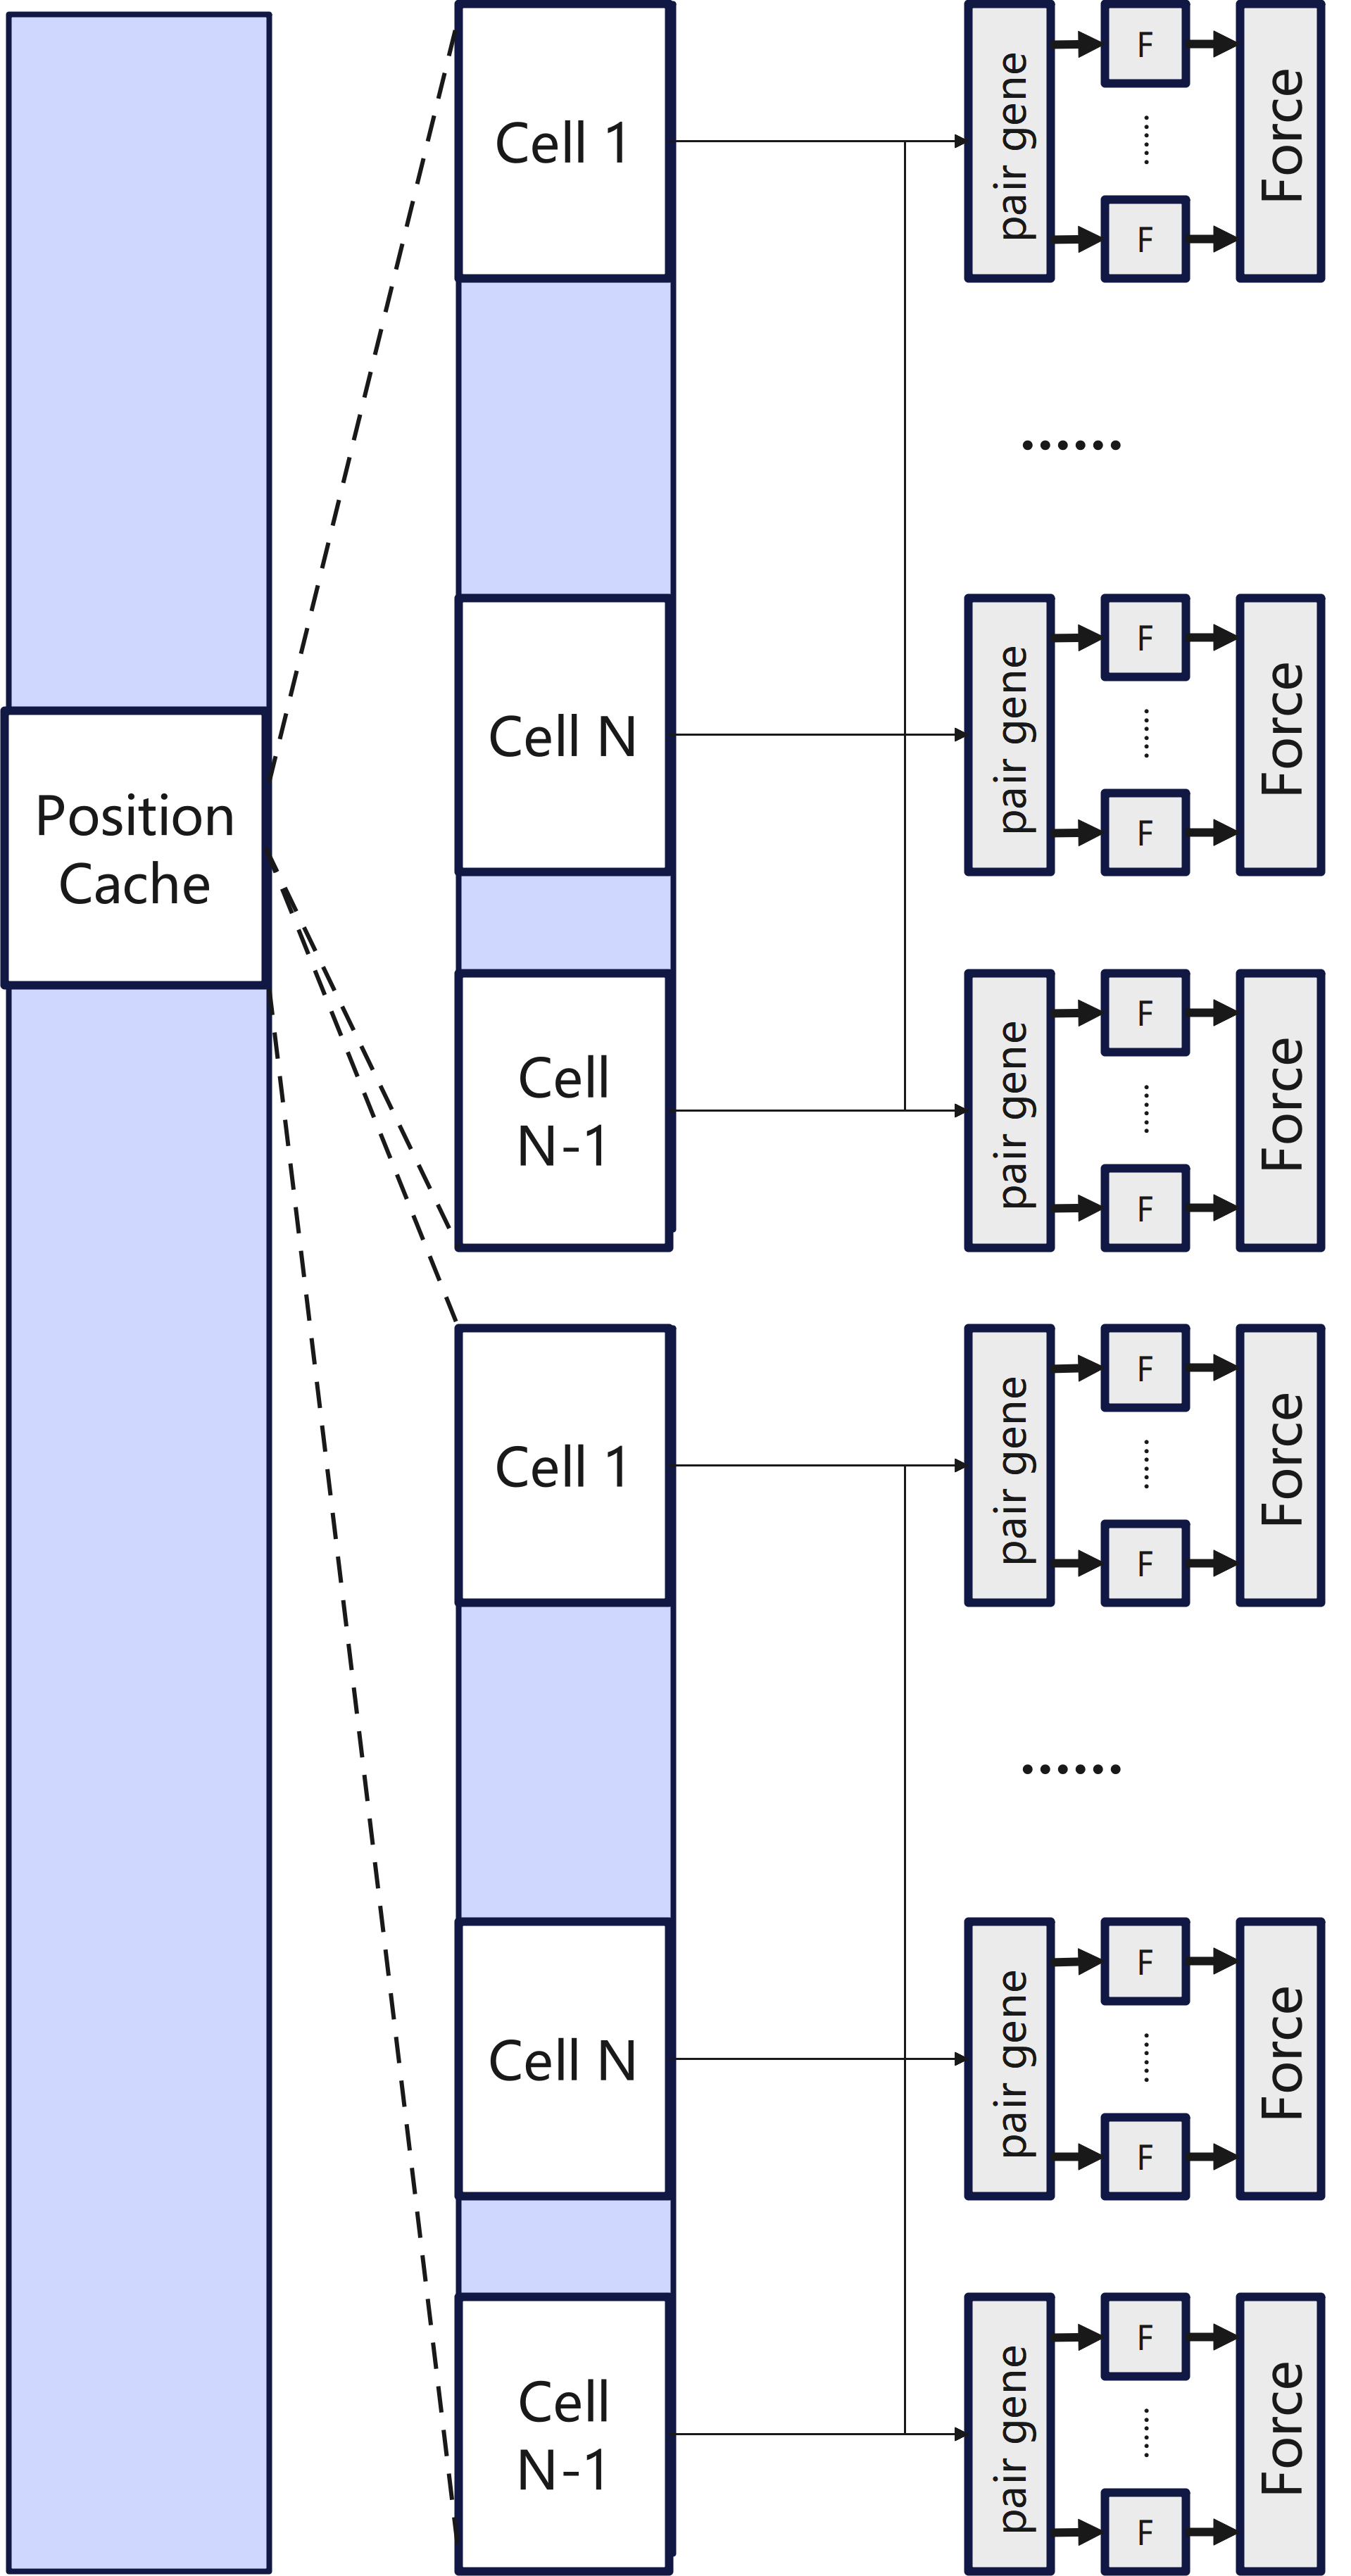
\includegraphics[width=0.3\textwidth]{./figures/Fig4_onecache.png}
		\label{fig:subfig1}
	}
	\subfigure[Data cached at the different address, multiple channels read simultaneously]{
		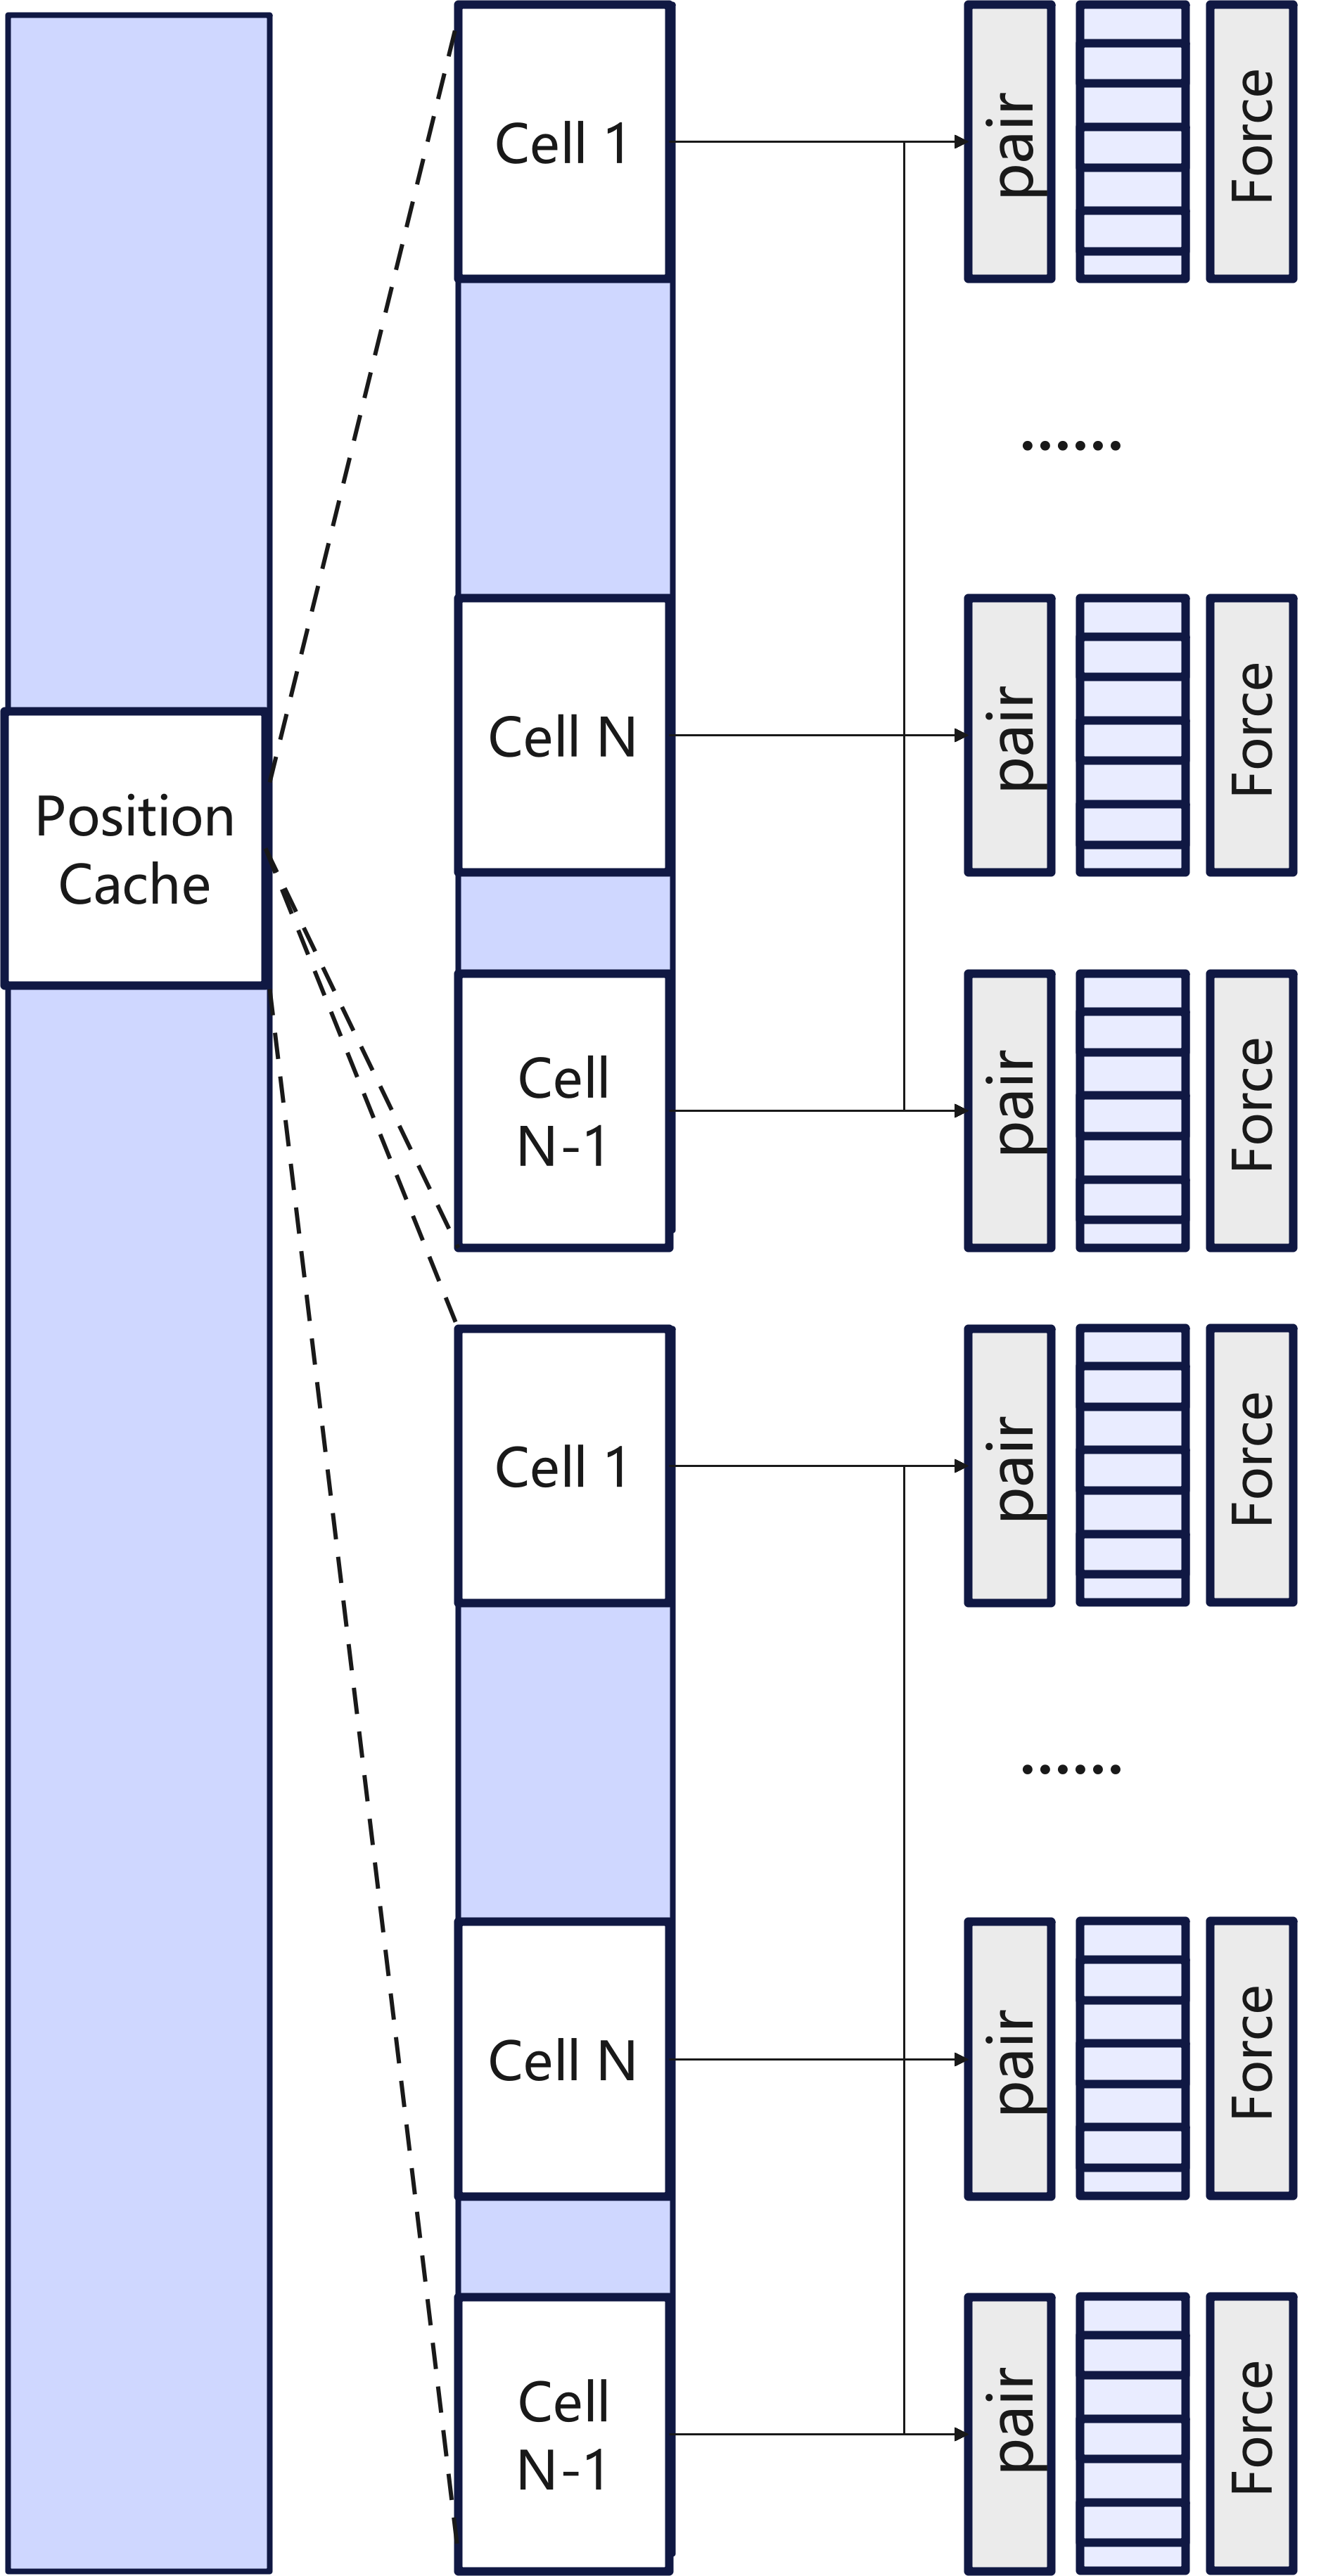
\includegraphics[width=0.3\textwidth]{./figures/Fig5_twocache.png}
		\label{fig:subfig2}
	}
	\caption{Data cached at the same address, multiple channels read simultaneously;Data cached at the different address, multiple channels read simultaneously}
\end{figure*}


\begin{sidewaysfigure*}[p]
	\centering
	\includegraphics[angle=0,width=0.9\textwidth]{./figures/Fig6_Upper_half_of_data_structures.png}
	\caption{(a),Particle information storage table Home Cell and Neighbor Cell storage relationship.
	      	 (b), The storage relationship between Home Cell and Neighbor Cell in the particle information storage table, the data length is 512 bits, and the data is mainly composed of six parts.
		     (c), the data structure of the particle information storage table Home Cell, the data length of the Home Cell is 512 bits bit width, and the non-data part needs to be zeroed in to facilitate the addressing
	      	 (d), particle pair computational information cache, data bit width is 256 bits bit width, since each Home Cell data is pre-computed with the first 13 Neighbor Cells}
	\label{fig:subfig3}
\end{sidewaysfigure*}

\begin{figure*}[!ht]
	\centering
	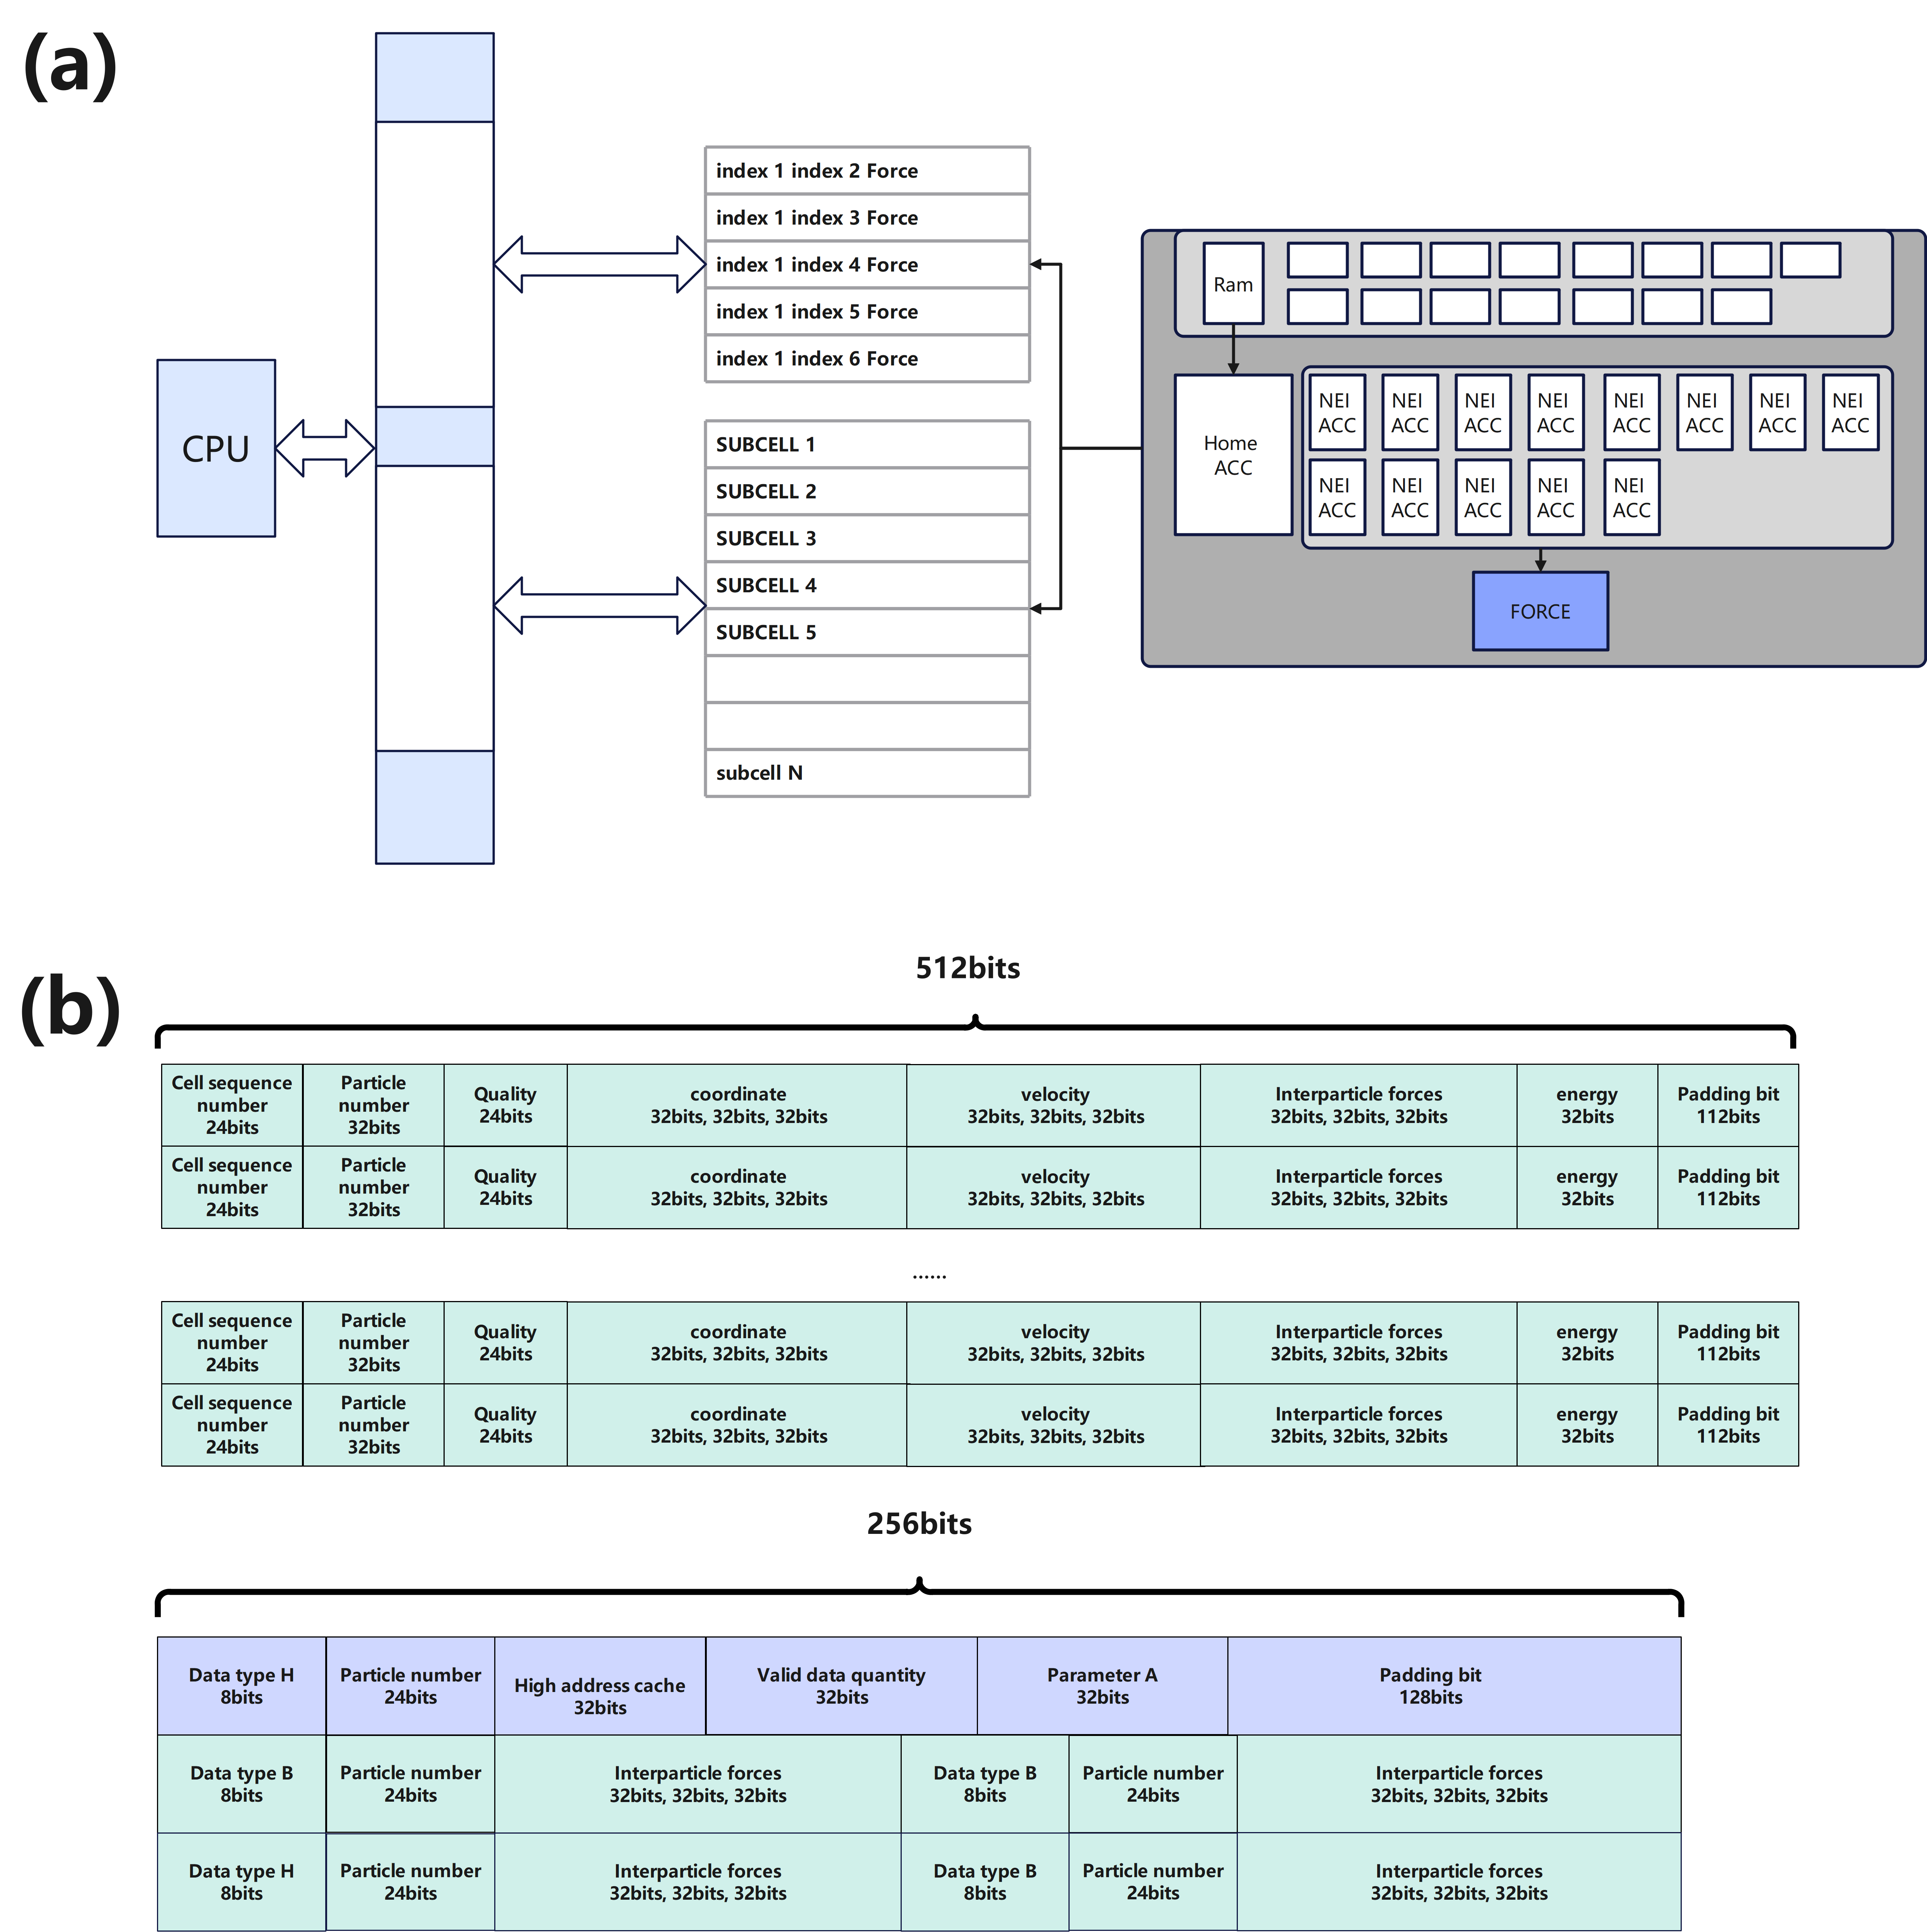
\includegraphics[angle=0,width=1.0\textwidth]{./figures/Fig7_lower_half_of_data_structures.png}
	\caption{(a), the Home Cell and the remaining 13 neighbor cells accumulate the results, and the data needs to be filtered a lot before the particles in the corresponding cell can   calculate the final short-range force.
		 (b), the block diagram of the storage structure of the RL force result buffer, the output of the calculation result of the particle pair, and the storage length of each particle information is 512 bits.Block diagram of the storage structure of the RL force result buffer, the output of the calculation result of the particle pair, the storage length of each particle information is 256bits, and the calculation result of each step is stored in a specific storage space, which is carried by the CPU for the remaining calculation processing.}
	\label{fig:subfig4}
\end{figure*}

\subsection{Generation of Interpolation and Coefficient Tables.}

\begin{figure}[!ht]
	\centering
	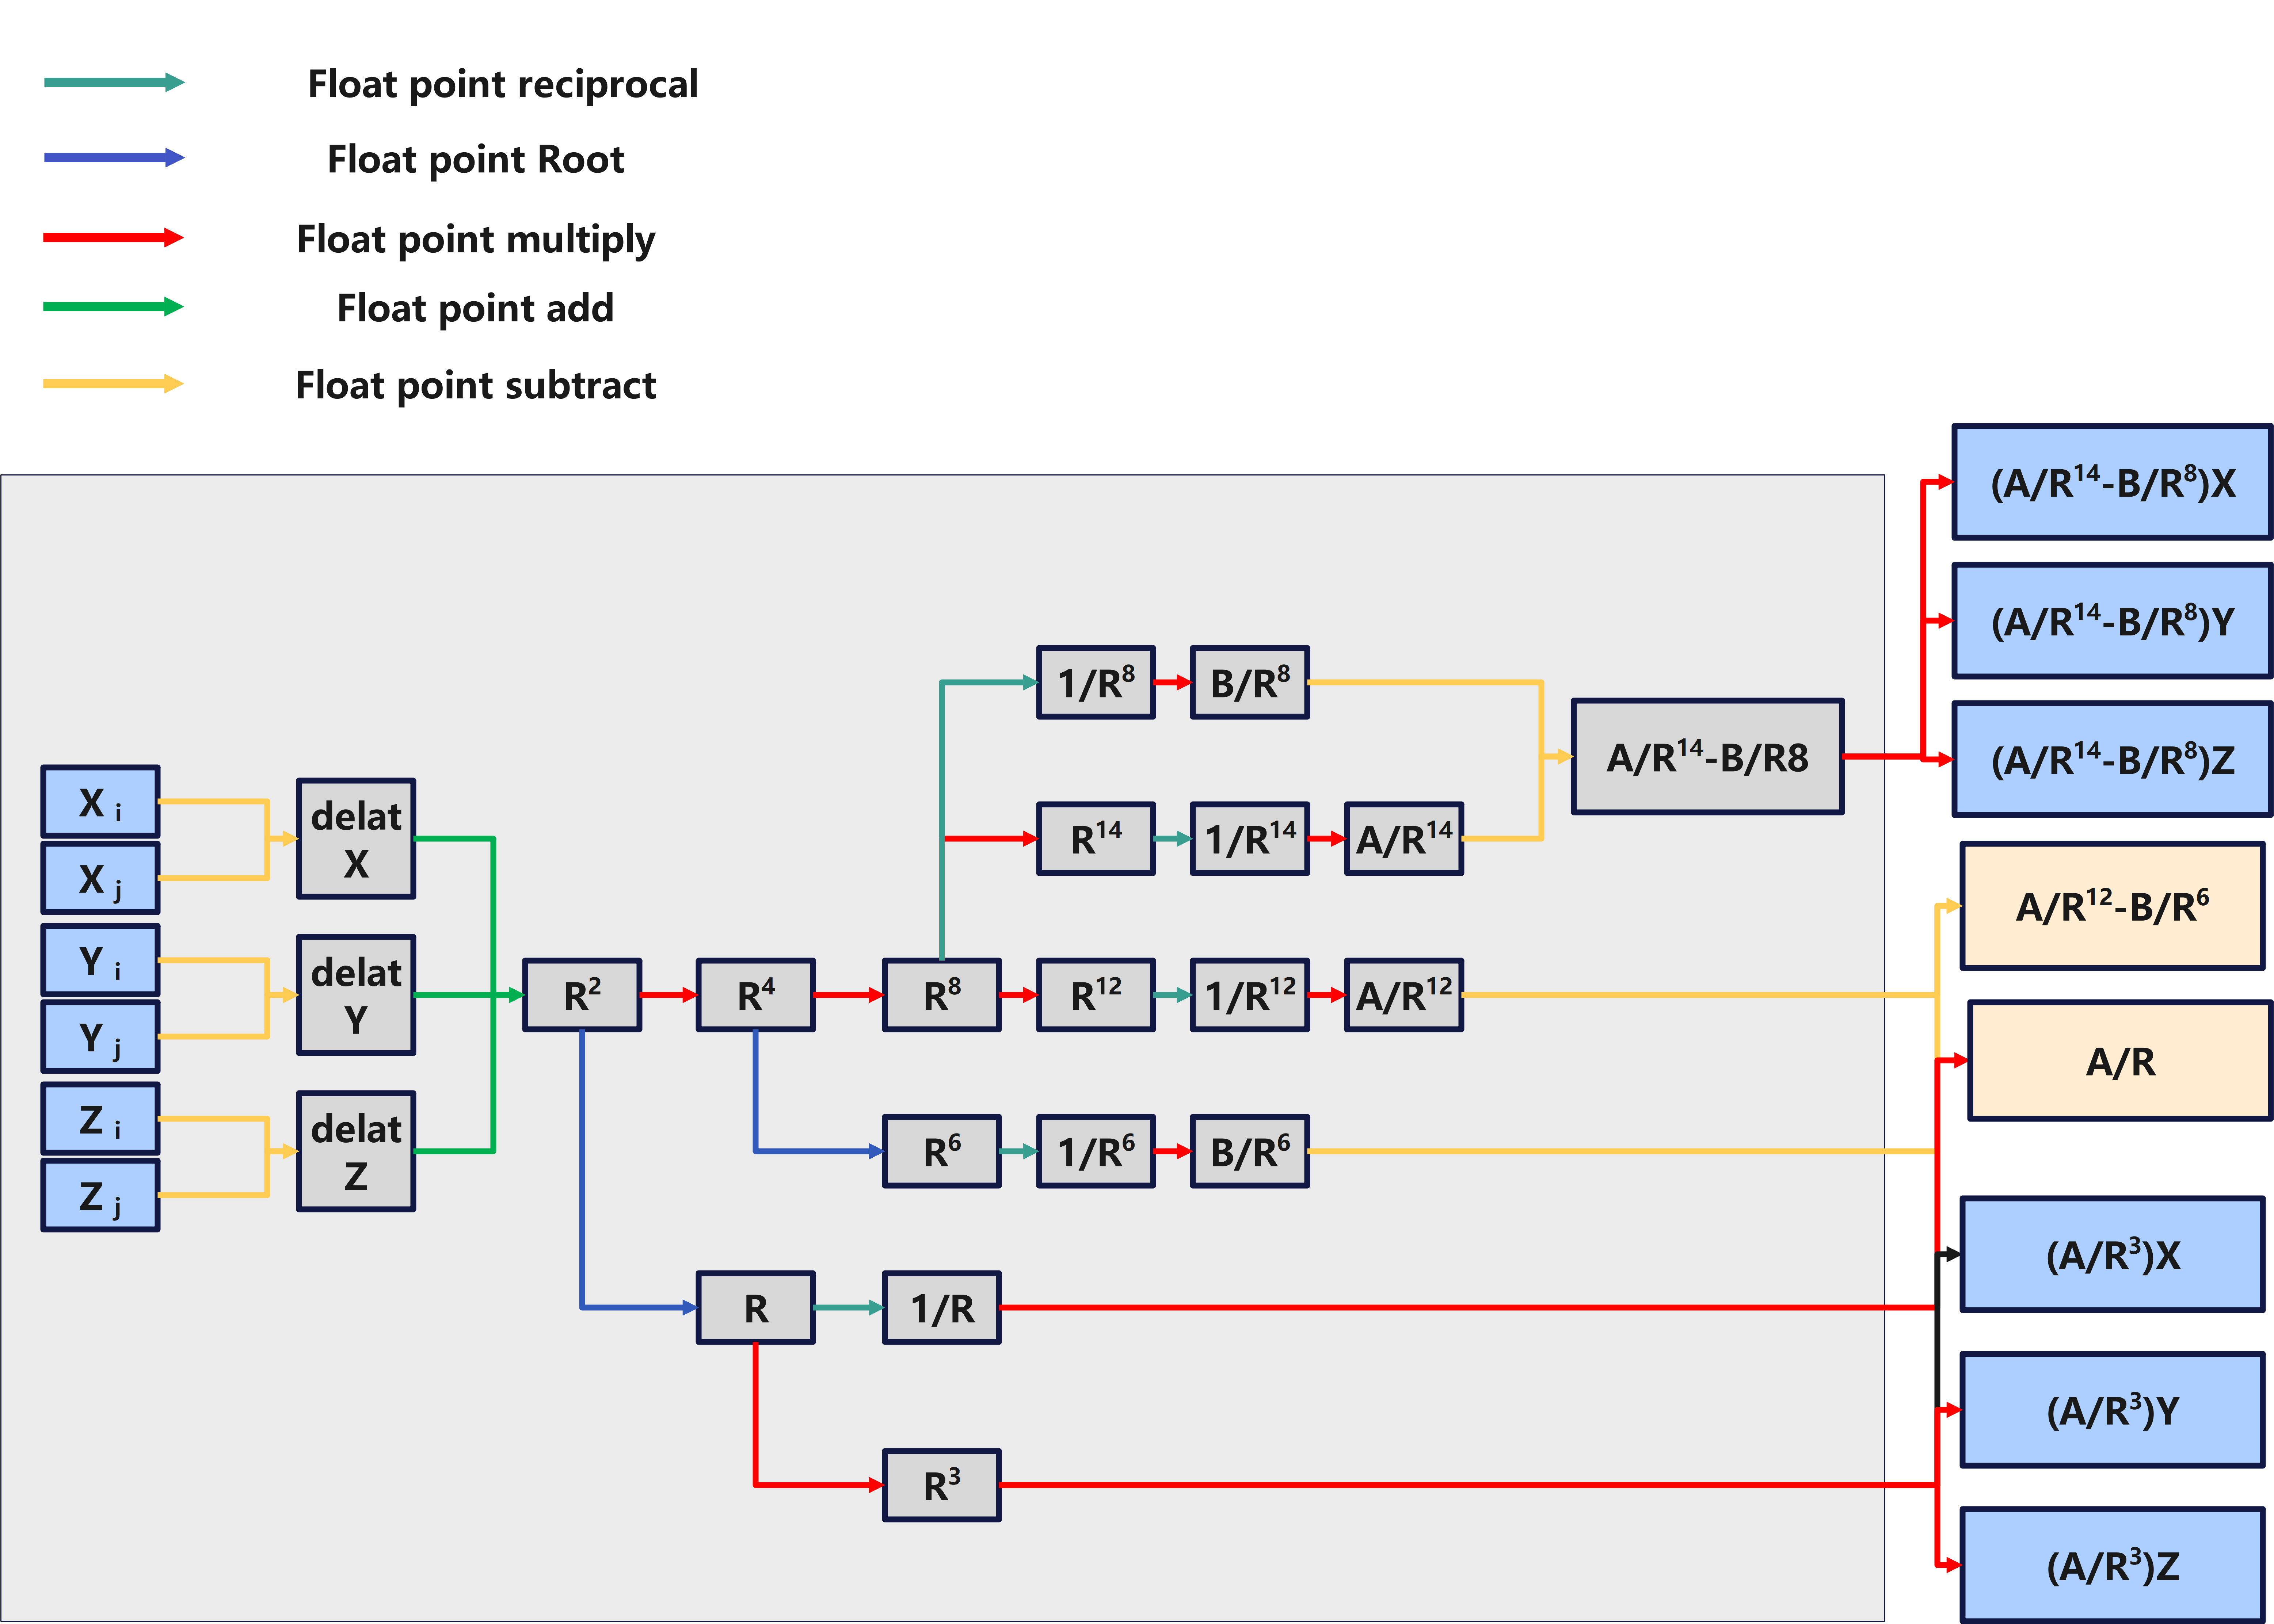
\includegraphics[angle=0,width=0.5\textwidth]{./figures/Fig8_force_direct_calculation_unit_module.png}
	\caption{The block diagram of the direct calculation module, assuming that particle i and particle j have gone through the particle screening module, and the short-range force of the particle pairs needs to be calculated within a certain range of action. The particle pairs are calculated directly by the DSP calculation pipeline, and the calculation results are single-precision floating-point numbers, which are calculated by the Xilinx floating-point number calculation unit, which is a relatively high-precision calculation method that consumes a large amount of DSP resources.}
\end{figure}

\noindent
Proximity force direct calculation unit module block diagram, assuming that 
particle $i$ and particle $j$ through the particle screening module, in a 
certain range of action need to calculate the short-range force of particle 
pairs, particle pairs through the DSP computing pipeline direct calculation, 
the calculation result is a single-precision floating-point number, using the 
Xilinx floating-point number calculation unit, this way of calculating the 
accuracy is relatively high, the consumption of DSP resources is more. 
The particles first go through the floating-point subtraction IP output 
multiplication IP to calculate 2. %??? 
In the hardware floating-point calculation, the root operation always consume a 
lot of logic resources, so we calculate the inter-particle interaction force, 
transform the formula form, and use 2 to do multi-level multiplication to 
calculate 14 and 8 in place of 13 and 7, which replaces the floating-point 
computation IP root operation. 
Using another lookup table to handle Coulomb force calculation pipeline, 
parallel computation does not interfere with each other in the computation 
time, the data is output to the last step after floating-point number 
multiplication and division calculation IP, and the corresponding particle 
parameters are read from the memory, such as A, B and other parameters in Figure. %???
After the calculation, the results for the LJ force and the Coulomb short-range force.
%???^

\begin{figure}[ht]
	\centering
	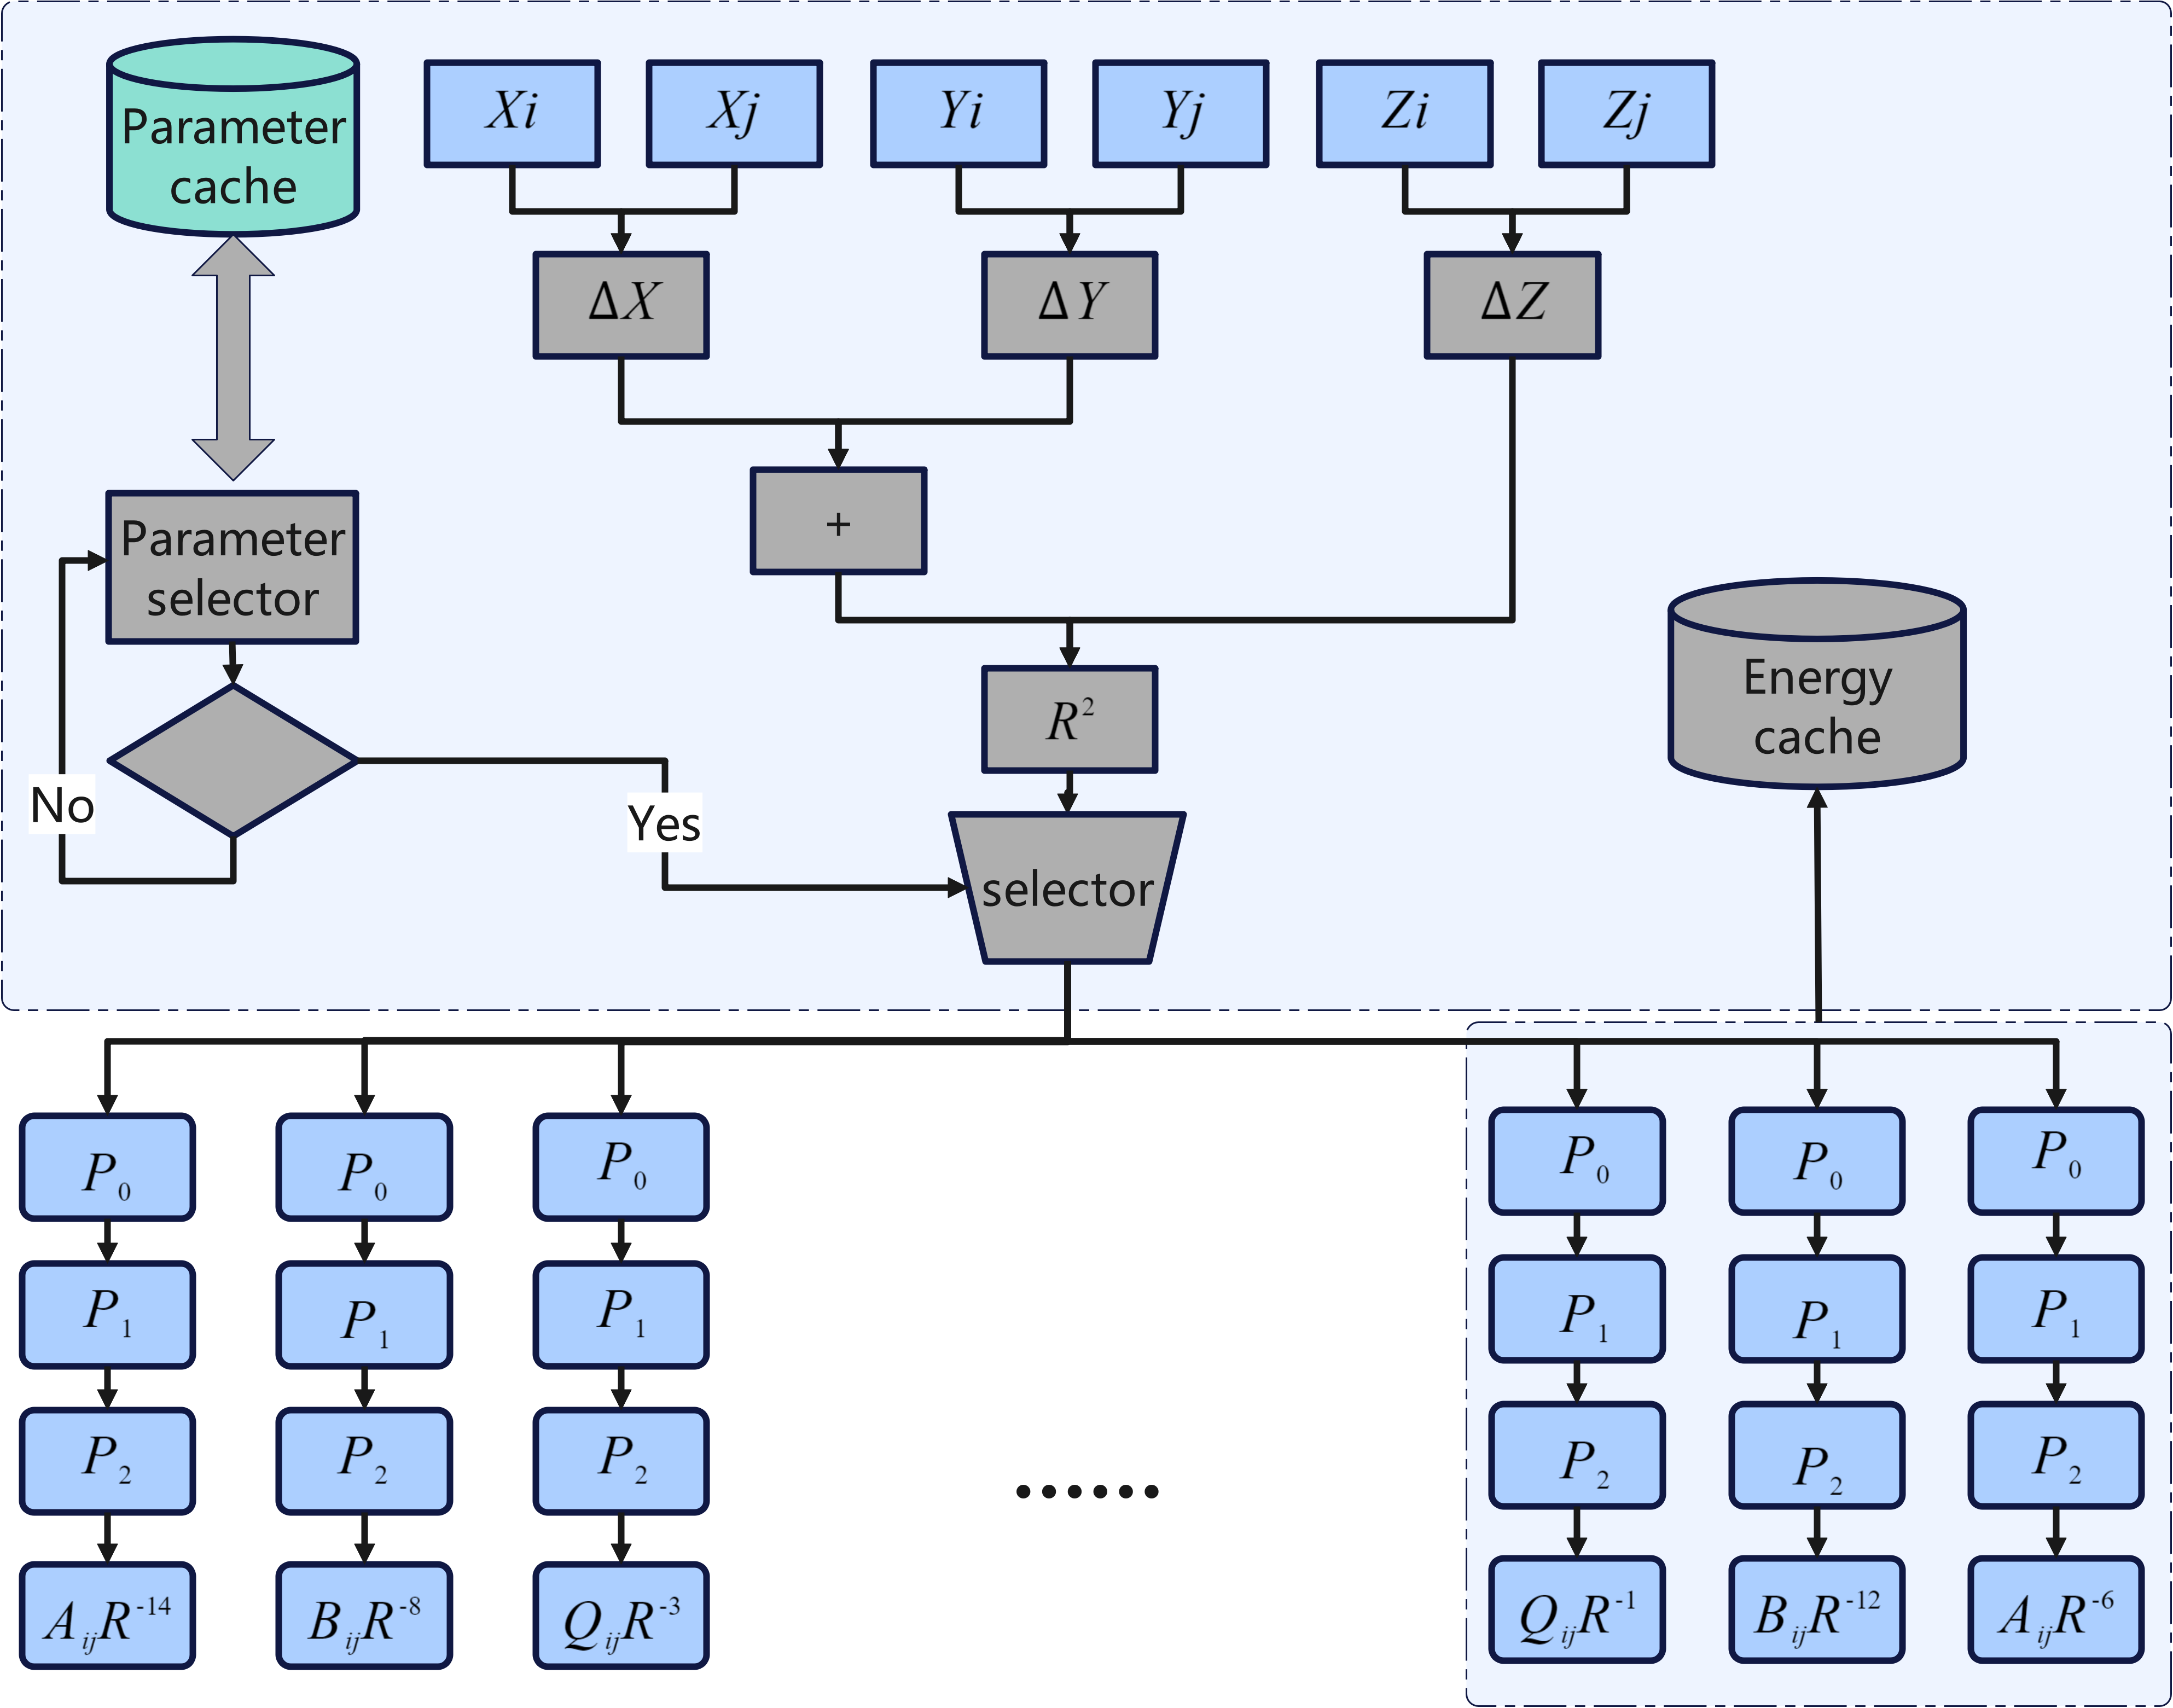
\includegraphics[angle=0,width=0.5\textwidth]{./figures/Fig9_Third_order_linear_interpolation.png}
	\caption{The figure shows the framework diagram of the second-order interpolation table DSP processing flow, the information of each particle is read from the parameter cache, after the arbitration of the parameter selector, the particle pairs go through the distance judgment, and the particles within the computation range enter into the force computation channel, assuming that the particles to be computed are particle i and particle j. }
\end{figure}

\noindent
% 距离这个可以删掉？
The design of the calculation module of the multi-channel calculation screener 
is realized as follows:
The calculation of the particle pair distance squared and the particle pair 
screening function is to include the 3D coordinates of the two particles in the 
information of the particle pair to be calculated, and the distance squared of 
the particles is equal to the sum of the squares of the differences of the 
coordinates in the three dimensions.\\

\begin{equation}
    r_{ij}^2 = ( x_{i} - x_{j} )^2 + ( y_{i} - y_{j} )^2 + ( z_{i} - z_{j} )^2 
\end{equation}

\noindent
% ???
The particle coordinates are represented using single-precision floating-point 
numbers, and $R^2$ is also stored using single-precision floating-point numbers.
The implementation of this formula is realized using floating-point arithmetic 
IP provided by the Xilinx manufacturer, together with auxiliary circuits to 
form a computational pipeline, where the distance squared for a set of 
particles can be computed for each clock. 
Since 2 has a limited range of values in the analog box and in making distance 
size comparisons, coefficient lookup tables, it is more convenient to use 
integers, all $R^2$ is uniformly enlarged by a certain factor, and then the 
integer part is taken for particle pair screening. particle pairs for which 
$R^2$ is smaller than the square of the truncated distance are selected as 
inputs to the subsequent calculations, otherwise ignored.\\

\noindent
%???
Otherwise, they are ignored. 
Since the spatial center distance of adjacent cells is greater than or equal to 
the truncation distance, there exists a certain probability distribution for 
the selected usable particle pairs. 
To maximize the arithmetic power, we use eight computation and screening 
modules working in parallel with three ports outputting at the same time, and 
the related table lookup operation is also allowed to look up the table at the 
same time according to the number of output ports.\\


\begin{equation}
    F^{RL}/r_{ij} = A_{ab} r_{ij}^{-14} 
                  + B_{ab} r_{ij}^{-8} 
                  + Q_{ab}r_{ij}^{-3}
\end{equation}
 
where, 

\begin{equation}
    A_{ab} = 48\epsilon_{ab}\sigma_{ab}^{12}
\end{equation}

\begin{equation}
    B_{ab} =-12\epsilon_{ab}\sigma_{ab}^6
\end{equation}

 
\begin{equation}
    Q_{ab} = \frac{q^a q^b}{4 \pi \varepsilon}
\end{equation}
  
  
In this design, $R^{-14}$, $R^{-8}$ and $R^{-3}$ are used in the formula of 
proximity force. 
In this design, $R^2$ is used as the output, and all the interpolating 
functions of the above three functions are created, which are reduced to 
low-order monic polynomials and then brought into $R^2$ to compute the 
original values, thus simplifying the computation process and reducing the 
consumption of DSP resources. 
The generation of the interpolating function should not only reduce the 
computational complexity, but also ensure that the accuracy of the computation 
meets the design requirements.

The $R^{-14}$, $R^{-8}$ and $R^{-3}$ can be fitted using a multi-order 
interpolation function of the form:


\begin{equation}
\begin{array}{c}
 f(x) = C_{0}+C_{1}(x-a)+C_{2}(x-a)^2 +C_{3}(x-a)^3 + \cdots \\ 
 + C_{p}(x-a)^p +o(x^p)
\end{array}
\end{equation}


After simplification, the accuracy requirement can be met by using 2nd- or 3rd-
order function fitting. 
The following equation shows the 3rd-order interpolation function form:
  

\begin{equation}
  F(x) = C_{0}+C_{1}x+C_{2}x^2 +C_{3}x^3
\end{equation}


Establish a reasonable interval, the interval sampling points of the formula 
erivative solution, you can get the corresponding interval of the fitting 
function. 
The following formula is a set of equations for the 2nd-order interpolation 
function to find the value of the interval $[x_{0}, x_{1}]$, for example, can 
be calculated to find the values of the 3 coefficients $a$, $b$ and $c$:


\begin{equation}
\begin{array}{c}
f(x_{0}) = cx_{0}^2 +bx_{0}+a\\
f^{'} (x_{0}) = 2cx_{0}  +b \\
f(x_{1}) = cx_{1}^2 +bx_{1}+a\\
f^{'} (x_{1}) = 2cx_{1}  +b \\
\end{array}
\end{equation}

%???
Assuming a fit to $R^{-14}$ with $R^{2}$ as the variable, the form of the 
equation can be simplified to $y( x ) = x^{-7}$.
The $y( x )$ function is monotonically decreasing in the range where x is 
greater than zero and very steep in the interval x( 0, 1]. 
The design requires values of $y( x )$ in the range $x [0.1, 144]$.
The greater the number of interpolation points and the smaller the intervals, 
the higher the computational accuracy, but the greater the number of segmented 
functions formed between the interpolation points, the larger the capacity of 
the coefficient table.
In addition, the higher the order of the interpolation function, the stronger 
the ability to track the function curve changes, the higher the accuracy, the 
more computing and storage resources consumed.
Therefore, we need to make a compromise according to the actual situation.
We use Python to compare and analyze the order of the interpolation function 
and the number and distribution of the interpolation points, and choose the 
second-order polynomial interface to meet the design requirements if the 
relative error is better than one-thousandth of a degree, and the polynomial 
library of Numpy provides the coefficients of polynomials fitting functions, 
which can be directly specified to the required order, and the results are 
comparable to those of the orthogonal polynomials such as Legendre's.
The results are similar to those of the orthogonal polynomials. 
The results are similar to those of orthogonal polynomials such as Legendre. 
Our final choice is the result of the calculation:

%???
The x interval is divided into 8 segments, as shown in the table, of which the 
first 7 segments, each segment is divided into 16 small segments, and the last 
segment, divided into 128 small segments, a total of 240 interpolation functions.
Each interpolation function requires 3 coefficients, expressed as 
single-precision floating-point numbers.
The interpolation table for each function can be fully stored using a 4KB BRAM.
The calculation of the proximity force also requires a table of coefficients 
for Aab and Bab, which need to be combined two by two for the particle types, 
so that if there are N independent particle types, the length of the table will 
be $N^2$ items. 
After analyzing the simulation dataset, there are no more than 
32 independent particle types, and the depth of the coefficient table is no 
more than 1024 items. 
The coefficients are expressed as single-precision 
floating-point numbers, and the coefficient table can be stored in 8 KB BRAM.
The inputs to the third-order interpolating proximity force calculation unit 
are all the parameters needed for the calculation formula, and the outputs are 
the three components of the force. 
Each clock cycle can input a set of 
calculation parameters, after the internal pipeline processing, each clock can 
output a set of settlement results. 
The following figure shows the realization 
'of the proximity force calculation unit block diagram.

\subsection{The make table module is used to calculate the process control.}

\noindent 
The particle computation oversight framework integrates multiple functional 
layers to optimize neighbor identification and force aggregation pipelines. 
A hierarchical memory architecture manages cell metadata through dynamic matrix 
structures: a 2D array (Module a) scales with system-wide cell populations to 
track neighbor indices per home cell, while a 1D auxiliary array (Module b) 
facilitates rapid index comparison and cross-referencing operations. 
A parallel comparison engine (Module c) evaluates eligibility criteria across 
these matrices using hardware-accelerated voting logic, enabling deterministic 
selection of interacting home cells based on spatial proximity thresholds.\\

\noindent
Sequence control is managed through a stateful counter array (Module d) that 
enforces strict access patterns to prevent memory coherence violations. 
Data retrieval from external high-bandwidth memory (HBM) is orchestrated by a 
pipelined fetch unit (Module e), which retrieves composite particle attribute 
blocks—each home cell requires 13 cumulative data segments including self and 
12 neighbor cells-through burst-optimized HBM controllers. 
The external storage subsystem (Module g) employs bank-interleaved addressing 
to resolve latency bottlenecks arising from concurrent access requests, while a 
data fusion module (Module f) aggregates force vectors from intra-cell and 
inter-cell interactions using SIMD-aligned accumulation registers.
This architecture achieves sub-microsecond neighbor search latencies through 
optimized matrix compression techniques and pipelined dataflow.\\

\begin{figure}[htp]
	\centering
	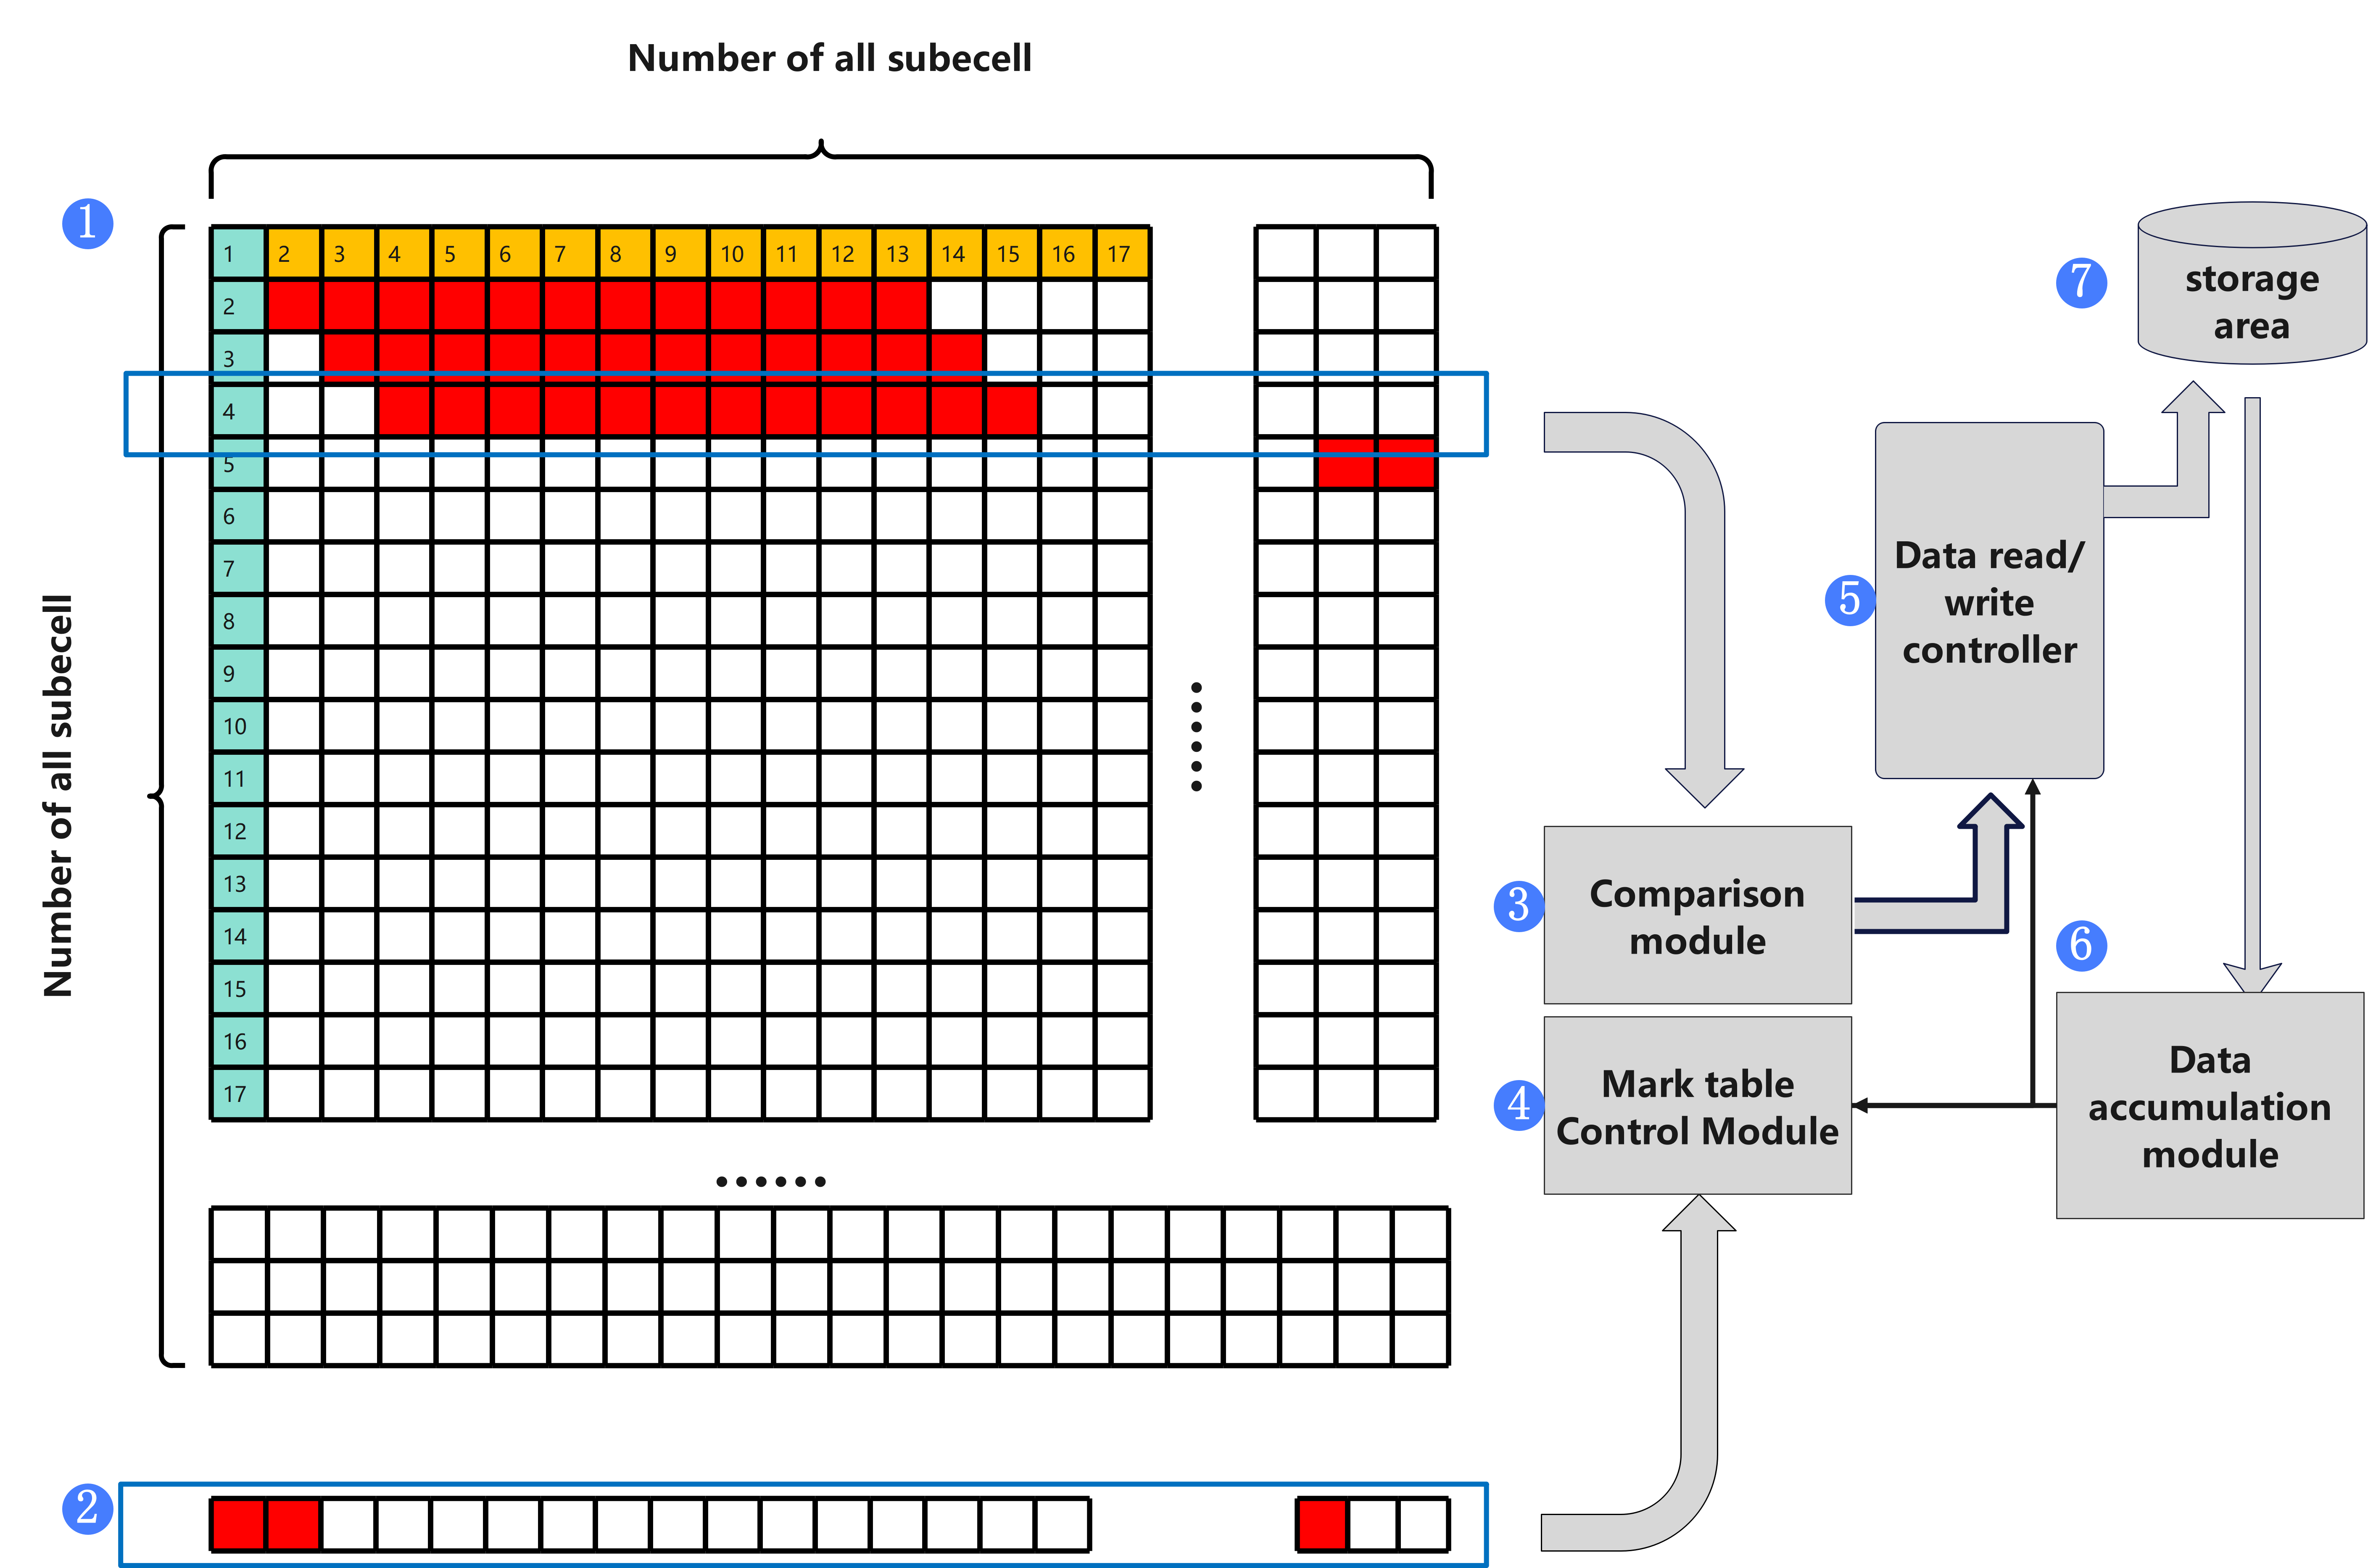
\includegraphics[width=0.7\textwidth]{./figures/Fig10_marktable.png}
	\caption{The particle computing progress monitoring module is composed of 
    several modules.}
\end{figure}


\subsection{3D Fourier transform.}
In this work, the computationally intensive 3D Fast Fourier Transform (FFT) 
module on an FPGA platform was implemented, while delegating remaining 
computational tasks to CPUs. 
Data exchange between the CPU and FPGA is facilitated through high-speed PCIe 
interfaces or optical fiber connections.
To accelerate Coulomb force calculations in MD, we developed a parallelized 
approach leveraging proximity lookup tables for Ewald summation, achieving 
parallelism comparable to vdW force computations.
% use ref in Figure
As illustrated in Figure 3-8, direct DSP channel implementations achieve 32-bit 
single-precision accuracy, with Figure 3-12 demonstrating 2nd-order 
interpolation structures for charge distribution. 
The simulation system undergoes cubic or rectangular grid partitioning 
along X/Y/Z axes, with grid dimensions determined by system boundaries to 
optimize hardware-accelerated data alignment. 
This design adapts simulation boxes to cubic/rectangular geometries for 
efficient data tiling. 
Temporal-spatial domain transformations employ optimized FFT algorithms for 
frequency-domain computations, while B-spline interpolation 
(order=3) maps particle charges to nearest grid points. 
Hardware implementation leverages OpenMM's reference codebase for kernel 
optimization, achieving 15$times$ speedup in Coulomb force calculations 
compared to CPU-only implementations when tested on the Inspur F37X platform. 
Resource utilization analysis reveals 83\% DSP block efficiency and 72\% HBM2 
bandwidth saturation during protein system simulations (100,000 atoms), 
demonstrating feasibility for large-scale MD workloads.

\begin{figure}[htp]
	\centering
	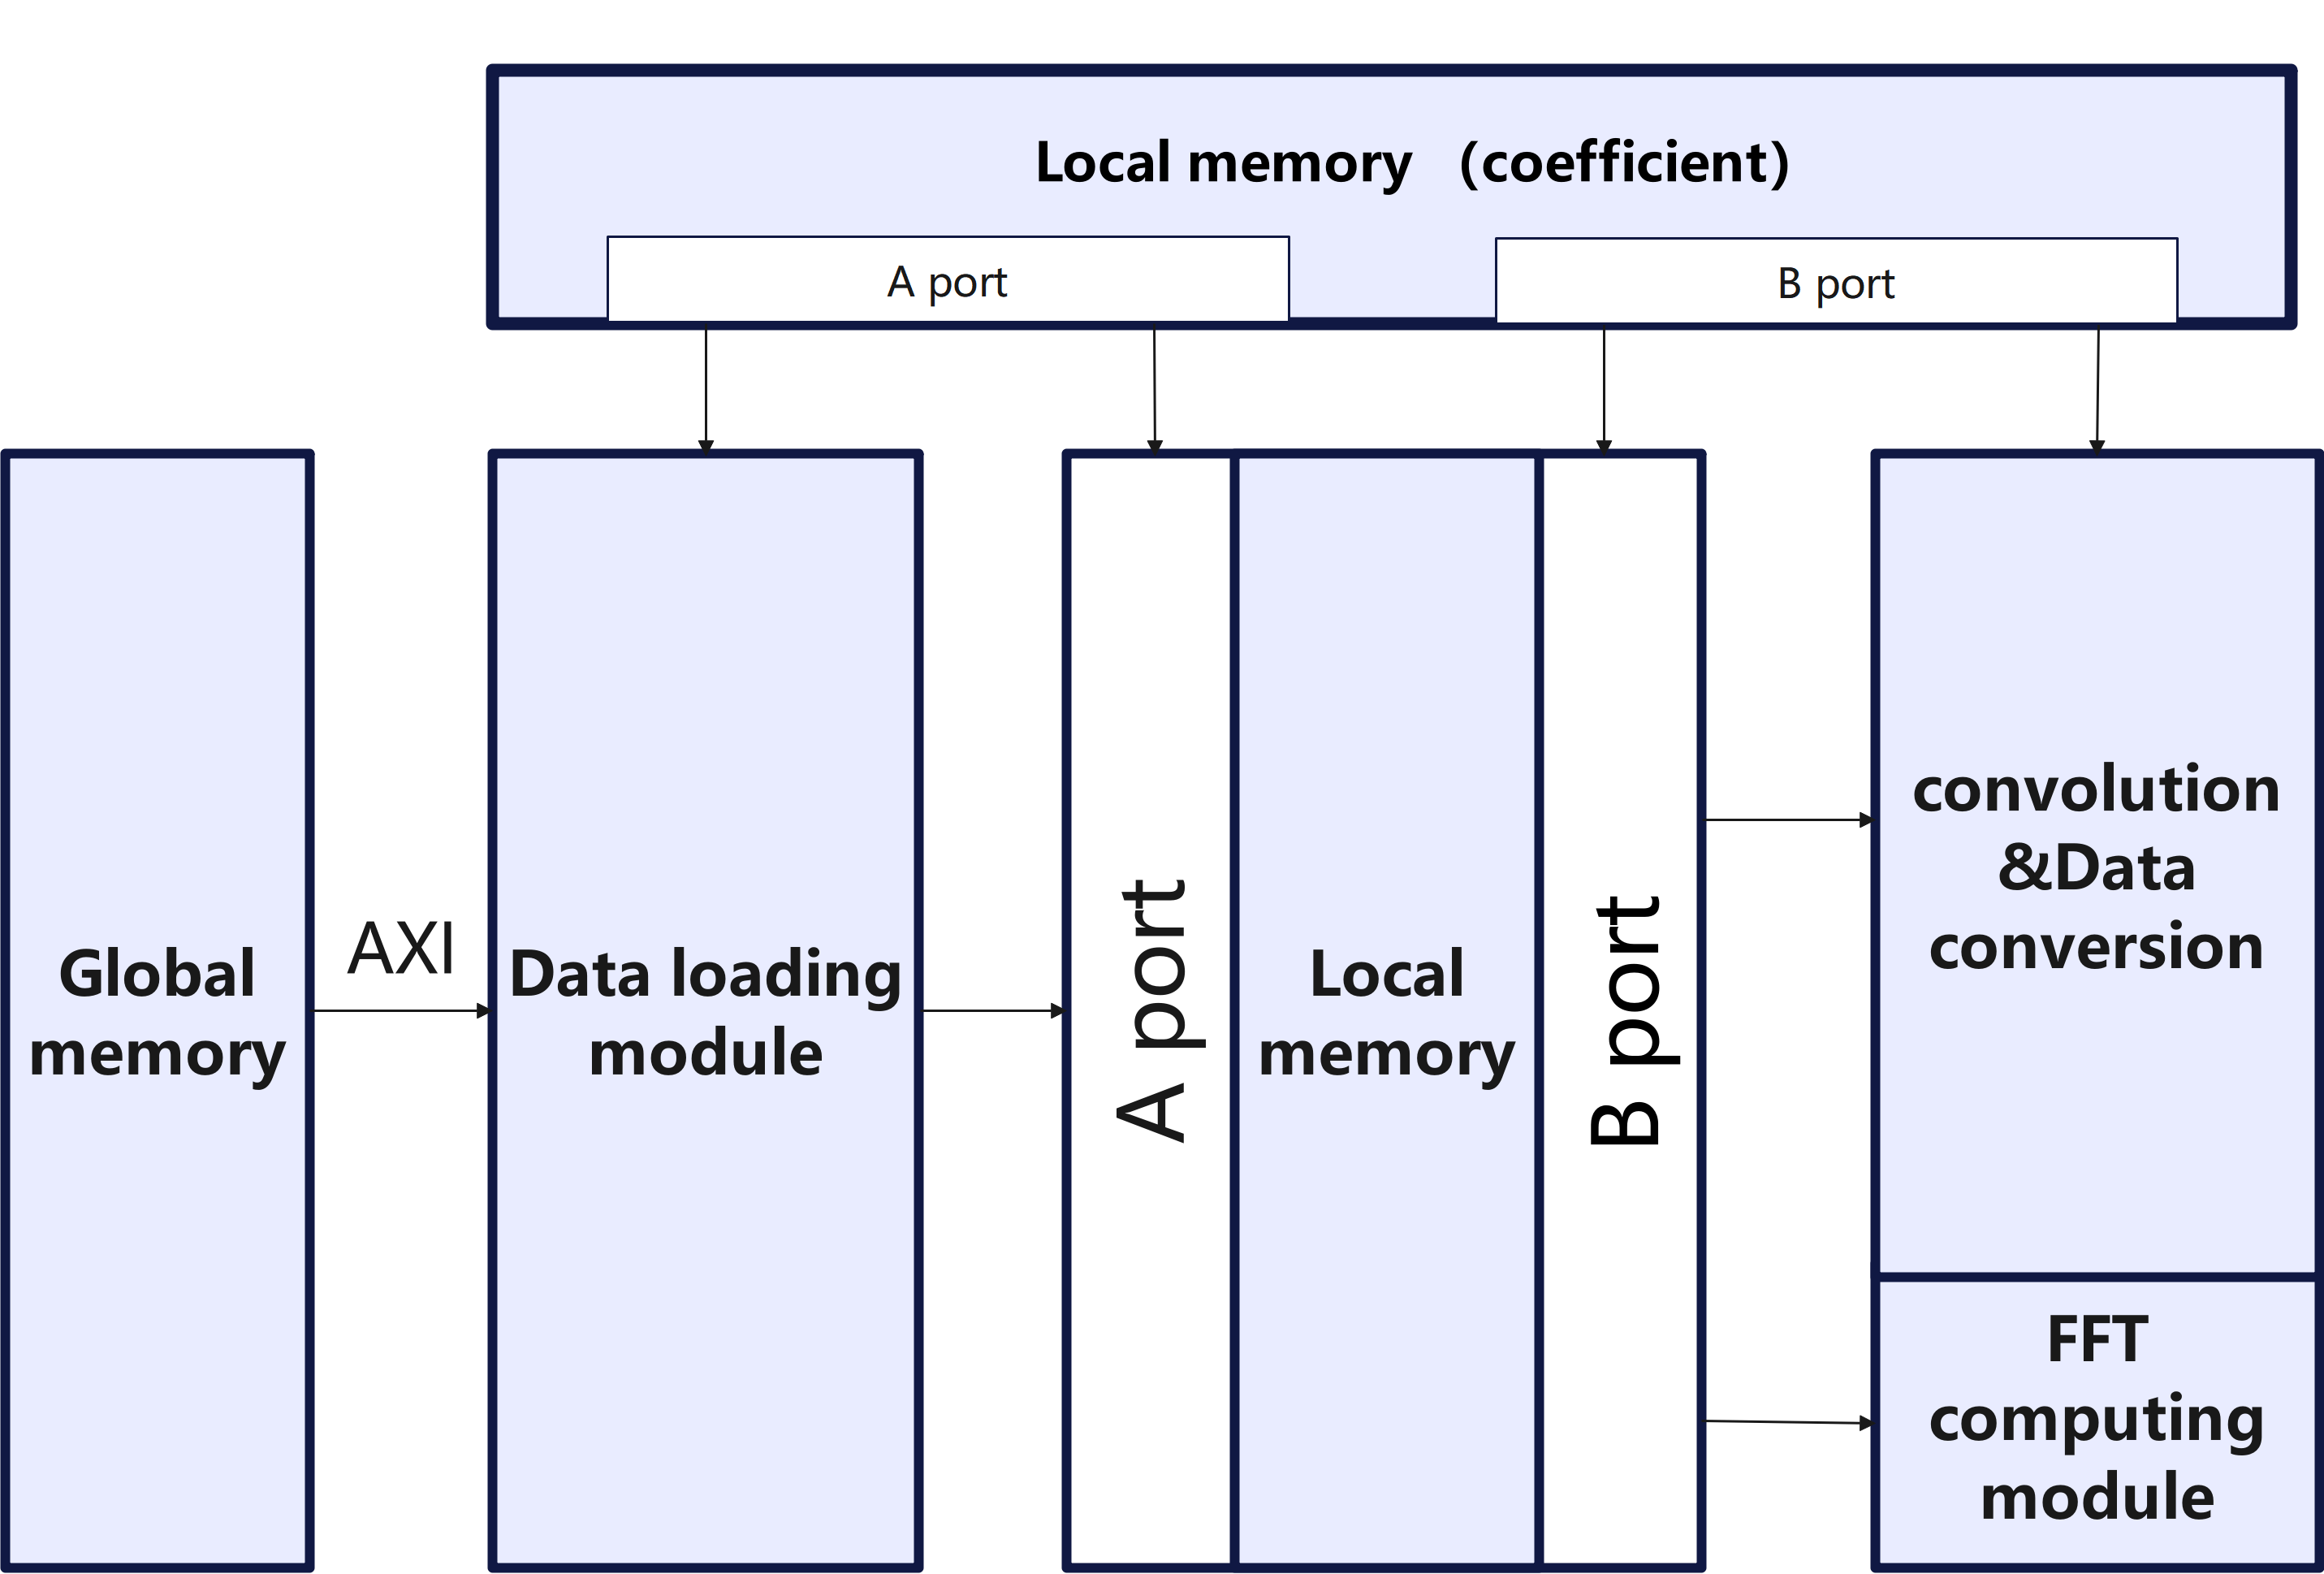
\includegraphics[width=0.7\textwidth]{./figures/3dfft_top_strcture.png}
	\caption{The 3D Fourier transform.}
\end{figure}


\subsection{Calculations of the bonded force and energy.}

Figure~\ref{fig:bond} shows the cooperation mode between CPU and FPGA in 
calculating the key force, and the data transmission between software and 
hardware is realized through PCIe 3.0. 
Each small box in the diagram represents a circuit processing unit. 
Particle information is derived from user input files, and the structure of 
particle information storage table is different for different user input files. 
% seems not neccessary
%This project uses FPGA as heterogeneous computing platform. 
%After receiving the particle bonding information provided by the user, the CPU 
%needs to carry out preliminary data processing.
%Because of different protein systems, it is necessary to construct 
%corresponding particle information table. 
This data is stored in a specific cache area of HBM2 using DMA technology. 
In classical MD simulations, bond topology describing how particles are 
connected remains unchanged during the simulation.

The FPGA data reading and writing submodule adopts multiple channels in 
parallel, and is equipped with HBM2 register, which can support multiple read 
and write operations simultaneously, therefore is able to read the interaction 
data between two, three and four bodies respectively.
This design greatly improves the storage and access efficiency of larger data 
blocks.

The computer flow control circuit is mainly responsible for the management and 
control of computer flow. 
In the force calculation, the process of the two-body force is relatively 
simple, so the calculation speed is faster. 
The calculated speed of the three-body force is between the two-body force and 
the four-body force. 
The calculation of the four-body force is the slowest, both in terms of the 
time required and the complexity of the process, which constitutes the main 
bottleneck in the whole calculation process.
Our covalent bond calculation buffer area, considering the access frequency of 
each calculation channel is different, in this design scheme, we set up a 
special circuit for receiving data from different channels. 
Only when all the data has been calculated will the subsequent calculation 
module be notified. 
% ???V
In the process of MD calculation, for some specific data, such as particles 
connected with hydrogen bonds, constraints such as the algorithm of unloading 
SHAKE algorithm to FPGA computing resource consumption can be used to limit. 
At this stage, we need to read the Index of these waiting bound particles.

\begin{figure}[htp]
	\centering
	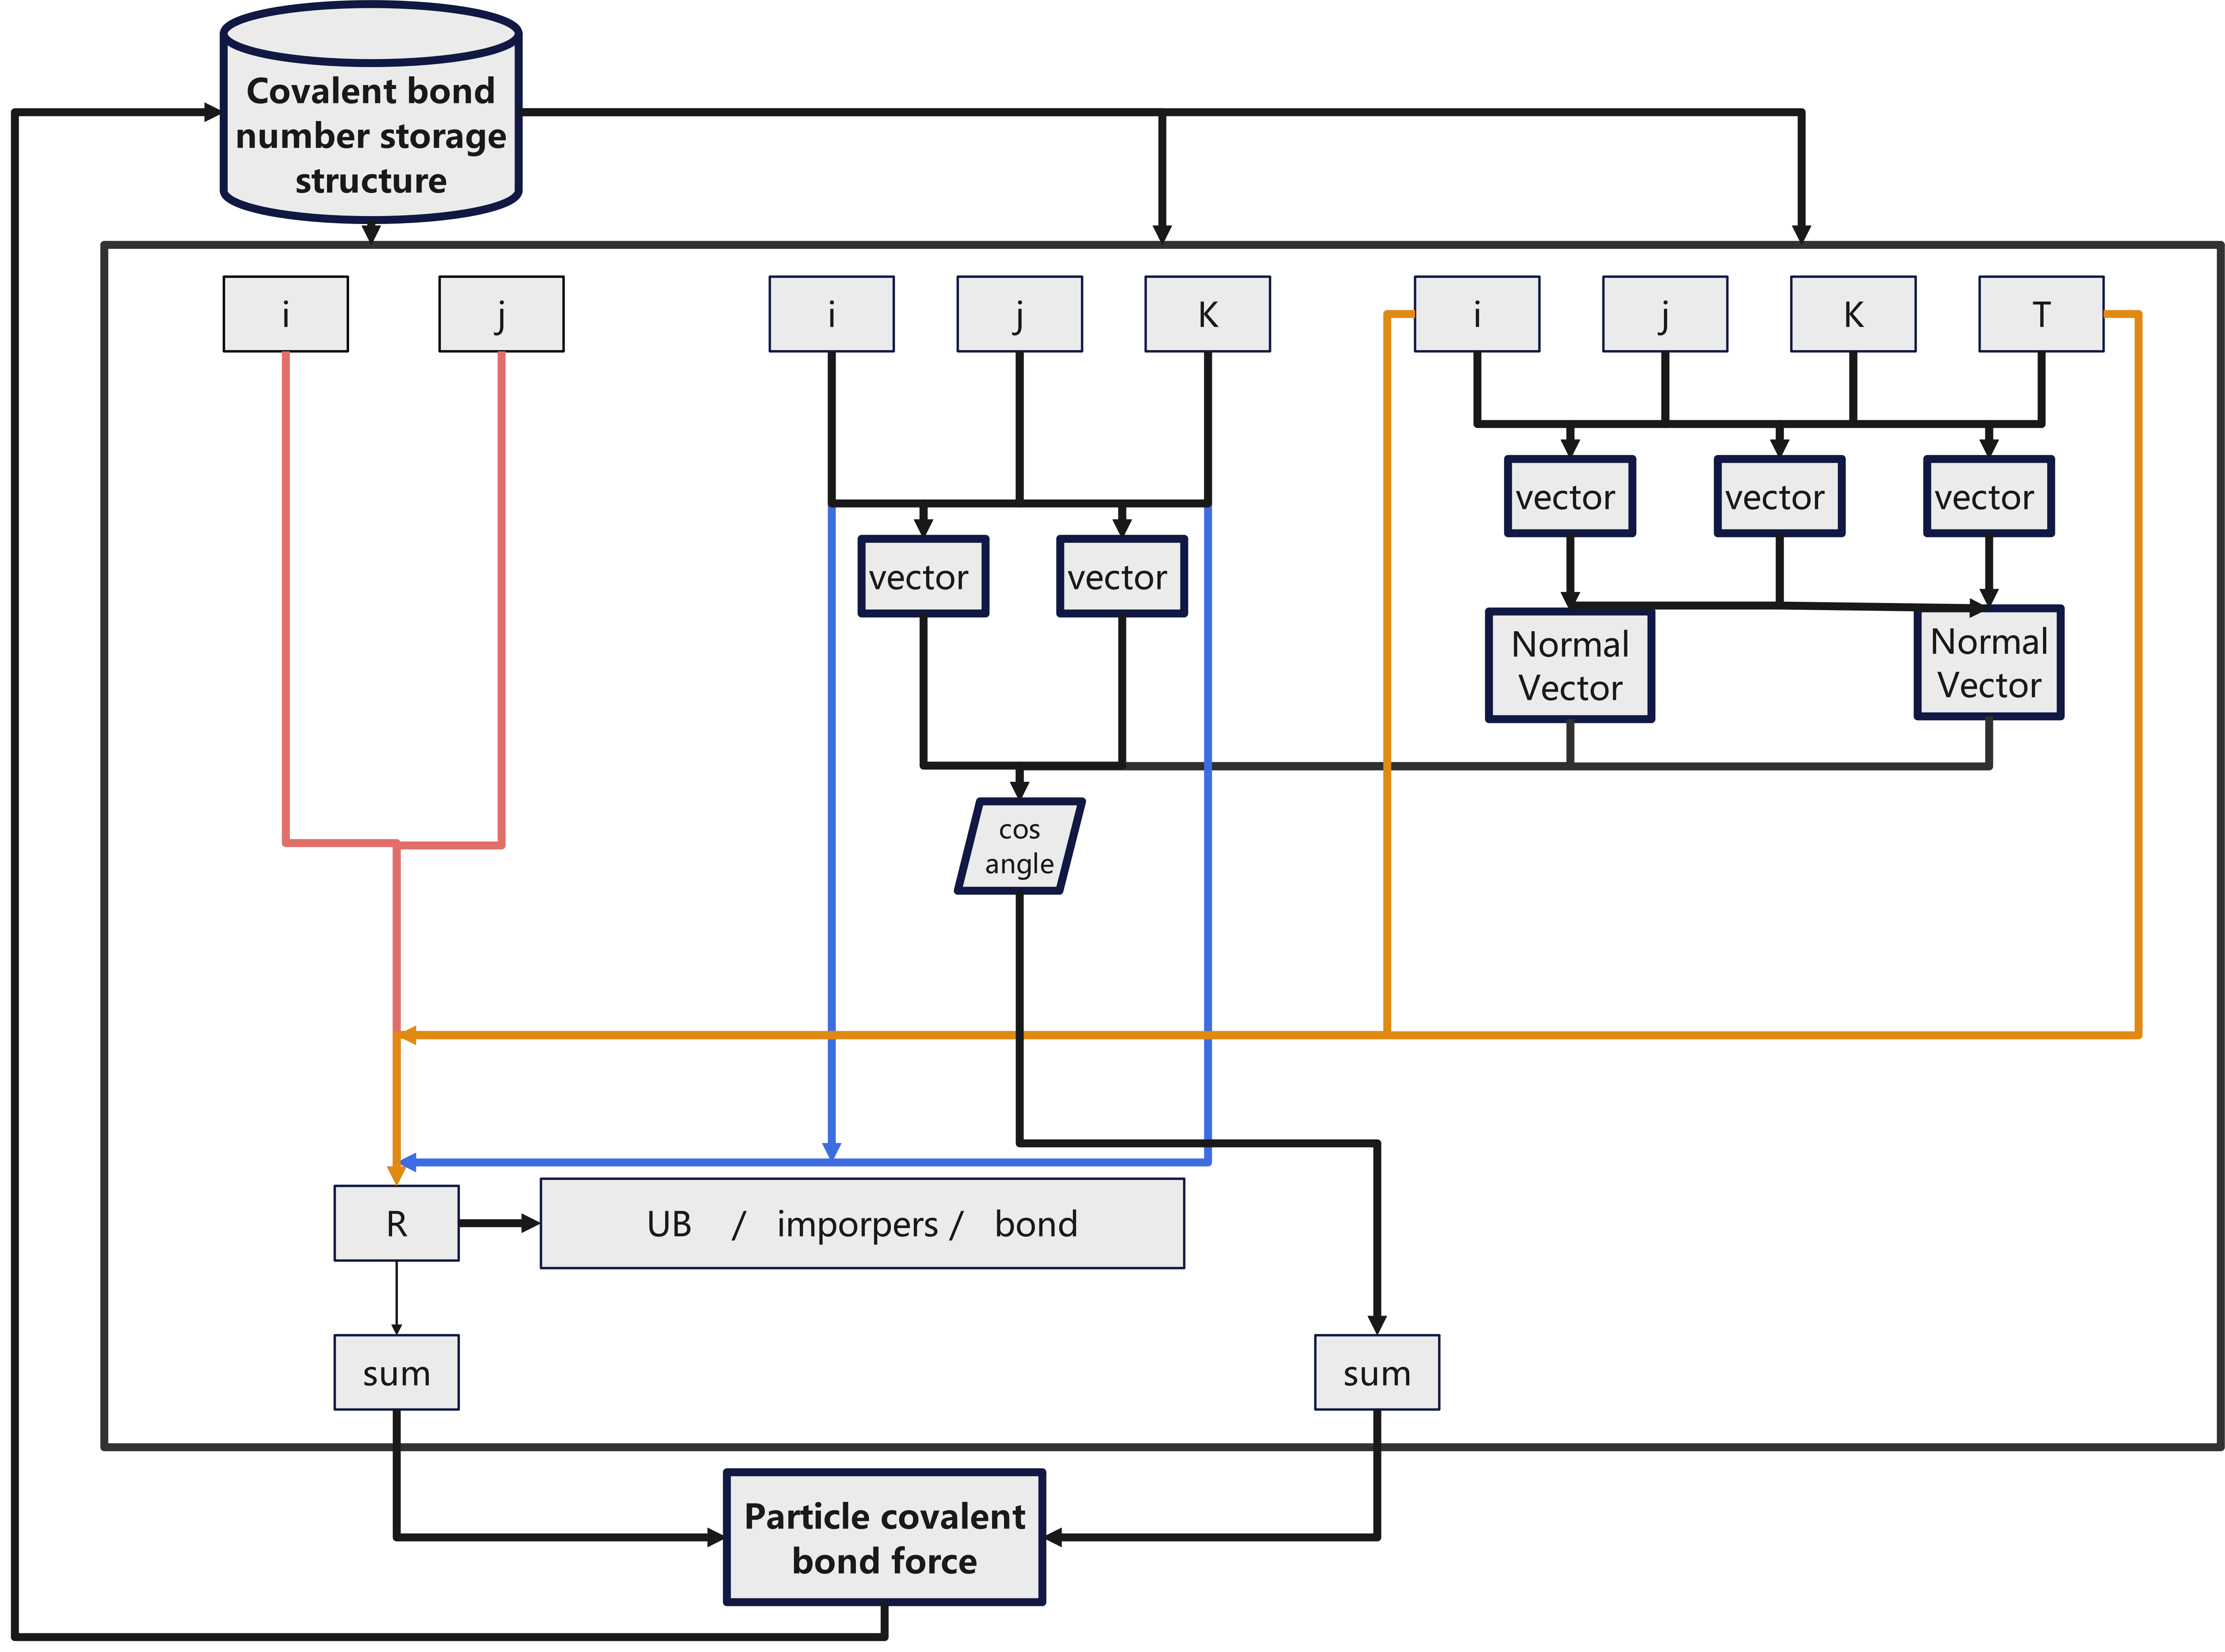
\includegraphics[width=0.7\textwidth]{./figures/Bond_force_calculation.png}
	\caption{
        The force of the covalent bond is calculated.
        These include two-force, three-force, four-force calculations, during 
        which a portion of the IP can be reused.}
	\label{fig:bond}
\end{figure}
\section{Results}

% TODO
The processing flow of data in the RL module is as follows: the CPU pre-processes the dataset of the MD simulation, and the pre-processed data will contain the following information, in which the cell serial number is obtained by segmenting the original data, and each particle will be assigned to a unique cell, and the particle information will be bound to the cell serial number to form the basic information of the particle to be processed. All other information in the data entry is obtained from the original data file. The side length of each data cell is determined based on the size of the truncation distance, and the number of data cells after CPU pre-processing is determined if the simulation data set exists in a deterministic rectangular space. Each data cell contains information about the particles it belongs to and the positions of the neighboring data cells, forming a data table to be stored in memorizer.

Each particle occupies one row of storage space. The length of the data cell is created according to the maximum number of particles after pre-processing, with an appropriate margin. Based on the serial number of the data cell, the starting position of the data cell can be directly located. Excluding particle information in pairs directly creates the structure shown in the following table. The number of excluded particles and their storage addresses are configured in registers for use by the relevant modules. The proximity force calculation requires the use of interpolation and coefficient tables, which are also prepared by the CPU and configured in the RAM of the FPGA. The information of the particle pairs to be excluded mainly comes from the existing co-bonded particle pairs, and the information of the two bonded particles is combined together to form the exclusion information data table, which is stored in the memorizer.

After the above configuration is completed, the CPU starts the prefetching particle data unit module to execute the next operation. The CPU can read the excluded particle information in parallel, and the particle reading module provides the particle pair information to be calculated.

Multi-Channel Calculation Filter Calculation Module, select each data cell as the main data cell in turn, take out the particle information of the main data cell and the particle information of the first 13 related data cells, take out a particle from the main cell, and take out one particle from each of the 13 neighboring cells, and form a particle pair to perform the distance calculation. Another particle is taken out from the main cell and formed into a particle pair with the current particle in the main cell for distance calculation. At this time, the current particle and 14 different particles are performing the distance calculation at the same time, and then based on the square of the distance calculation result and the square of the truncated distance, the particle pair smaller than the truncated distance is selected for the subsequent calculation. The coefficients of the interpolation table are obtained by querying the interpolation table based on the squared distances of the selected particle pairs, and the coefficients are obtained by checking the table based on the particle type information of the particle pairs. The coefficient values are based on the charge information in the FPGA which is needed for the calculation of the electrostatic force and the short-range force. At the end of the table, all the parameters for calculating the limited range force are obtained, and all the information is stored in the FPGA on-chip RAM and passed to the particle distance judgment module for screening, and only the particles within the distance range are allowed to carry out the next step in the force calculation pipeline. The calculation progress of the particles is passed to the proximity force calculation monitoring module, which is used to update the proximity force calculation result data table and supervise the progress of calculator calculation.

\subsection{High-Level Language Synthesis (HLS) Design Experiment Results}

The HLS compilation tool optimizes DSP resources, and we focus on testing the performance optimization effect of particle-to-computation units, using the HLS synthesis tool for first-order linear interpolation.

Using Xilinx's HLS for the multiply-add implementation of second-order polynomials, the synthesis results in the use of four floating-point IPs (two multipliers and two adders) for a total of 10 DSP48 modules. With a clock constraint of 300MHz, the pipeline optimization requires 22 clock cycles to complete the implementation.
If the clock constraint is 200MHz, it takes 18 clock cycles for Pipeline to complete the function.
To ensure the accuracy of the calculation and consider the range of values of the coefficient table, it is not worthwhile to convert the fixed-point realization.
Regardless of the implementation method, if Xilinx's floating-point computing IP is ultimately used, the performance and resource usage can be expected to be comparable.
The calculation of the square of the distance between two particles consumes approximately 19 DPS48 modules and takes 25 clock cycles.

Each RL module uses approximately one $R^2$ computational unit for particle pair screening, three computational units for interpolating polynomials and one force merger accumulator for force vector computation, and a number of accumulators for accumulating force vectors of neighboring cells.


\begin{table*}[!ht]
	\centering
	\begin{tabular*}{\hsize}{@{}@{\extracolsep{\fill}}llllllll@{}}
		\toprule
		Modules&Latency(cycles) & Latency(ns) & DSP &FF &LUT \\\\ 
		\midrule
	First Order Linear Interpolation Modules 
        &22 &73.304 & 10 & 1459 & 763\\\\
        Second Order Linear Interpolation Module &34 &113.288 & 16 & 1788 & 1063\\\\
        Third Order Linear Interpolation Module &45 &148.514 & 22 & 2442 & 1452\\\\ 
	\bottomrule
	\end{tabular*}
	\caption[Performance and Resource Evaluation]{Performance and resource evaluation of multiplication and addition of first-order polynomials using Xilinx's HLS, totaling 10 DSP48 modules. With a clock constraint of 300MHz, Pipeline requires 22 clock cycles to complete the functional implementation. The performance and resource evaluation of multiply-add second order polynomials using Xilinx's HLS is performed on a total of 16 DSP48 modules. Pipeline requires 34 clock cycles to complete the functional implementation; Xilinx's HLS is used to evaluate the performance and resources of the multiply-add operation for third-order polynomials, totaling 22 DSP48 modules. With a clock constraint of 300MHz, Pipeline requires 45 clock cycles to complete the function}.
\end{table*}


\begin{table*}[!ht]
	\centering
	\begin{tabular*}{\hsize}{@{}@{\extracolsep{\fill}}llllllll@{}}
		\toprule
		Type &Module 2 utilization rate\%&Module 1 utilization rate\%  \\ 
		\midrule
		LUT &10 & 21 \\ 
		LUTRAM & 3 & 6  \\ 
		FF & 13.13&  26.4 \\ 
		BRAM & 7 & 18.5 \\ 
         URAM & 0.63 & $\sim$\\ 
		DSP &2& 4  \\ 
		IO & 1  & 1 \\ 
		GT & 17 & 34   \\ 
		BUFG & 3  & 6 \\ 
		MMCM & 8  & 16 \\ 
		PLL & 17 & 34 \\  
		\bottomrule
	\end{tabular*}
	\caption {The FPGA platform was Xilinx Virtex UltraScale+ VU37P with Inspur F37X.Comparison of resources used by a single module and two RL modules in finite range.}
\end{table*}


\begin{table}[!ht]
	\centering
	\begin{tabular*}{\hsize}{@{}@{\extracolsep{\fill}}llllllll@{}}
		\toprule
		Resource Name & Utilization\%  \\
		\midrule
		LUT & 16  \\ 
		LUTRAM & 4  \\ 
		FF & 14 \\ 
		BRAM & 58 \\ 
		DSP & 7  \\ 
		IO & 1  \\ 
		GT & 17  \\ 
		BUFG & 2  \\ 
		MMCM & 8  \\ 
		PCIe & 17  \\ 
		\bottomrule
	\end{tabular*}
	\caption[64-bit sequence resource utilization based on BRAM bar chart]{Layout routing uses Xilinx Virtex UltraScale+ VU37P chip, FFT 64-bit sequence resource utilization based on BRAM bar chart.  }
\end{table}


\begin{table}[!ht]
	\centering
	\begin{tabular*}{\hsize}{@{}@{\extracolsep{\fill}}llllllll@{}}
		\toprule
		Resource Name & Utilization\%  \\ 
		\midrule
		LUT & 15  \\ 
		LUTRAM & 4  \\ 
		FF & 14 \\ 
		BRAM & 24 \\ 
		URAM & 13 \\ 
		DSP & 7  \\ 
		IO & 1  \\ 
		GT & 17  \\ 
		BUFG & 2  \\ 
		MMCM & 8  \\ 
		PCIe & 17  \\ 
		\bottomrule
	\end{tabular*}
	\caption[64-bit sequence resource utilization based on URAM bar chart]{Layout routing uses Xilinx Virtex UltraScale+ VU37P chip, FFT 64-bit sequence resource utilization based on URAM bar chart.  }
\end{table}

\begin{table}[!ht]
	\centering
	\begin{tabular*}{\hsize}{@{}@{\extracolsep{\fill}}llllllll@{}}
		\toprule
		Resource Name & Utilization\% \\
		\midrule
		LUT & 15 \\
		LUTRAM & 4 \\
		FF & 14 \\
		BRAM & 24 \\
		URAM & 13 \\
		DSP & 3 \\
		IO & 1 \\
		GT & 17 \\
		BUFG & 2 \\
		MMCM & 8 \\
		PCIe & 17 \\
		\bottomrule
	\end{tabular*}
	\caption[Resource utilization of RTL covalent bond module]{Resource utilization rates for covalent bond module implemented on Xilinx Virtex UltraScale+ VU37P chip through layout routing.}
\end{table}


\begin{table}[!ht]
	\centering
	\begin{tabular*}{\hsize}{@{}@{\extracolsep{\fill}}llllllll@{}}
		\toprule
		~ & Model & Clock Frequency & 32×32×32 (µs) & 64×64×64 (µs) \\
		\midrule
		FPGA & VU37P & 300MHz & 18.33 & 119.7 \\
		NVIDIA\cite{8056853} & Tesla K20c & 0.73GHz & 29 & 92 \\
		Anton\cite{anton1} & ~ & ~ & 4 & 13 \\
		\bottomrule
	\end{tabular*}
	\caption[Performance comparison of 3D FFT computation module at different clock frequencies]{Implementation of 3D FFT computation module using Xilinx Virtex UltraScale+ VU37P accelerator card. The module completes data reading, 3D FFT computation, convolution, inverse transform, and data storage. Pipelined mode is configured for testing. Input data includes single-precision floating-point matrices of dimensions 32×32×32 and 64×64×64.}
\end{table}

The FFT computation module contains 4 FFT computation kernels, each kernel includes 8 FFT computation channels, capable of parallel computing 32 one-dimensional FFTs per clock cycle. Each plane requires two one-dimensional FFT computations, and 64 planes require 128 one-dimensional FFT computations. As shown in the FFT 9.0 user manual \cite{8056853}, the pipelined mode offers the fastest speed but increases resource consumption exponentially. The following tables use pipelined mode testing.

Global memory stores 32-bit static potential real parts and coefficients with 256-bit bit width (32×8), requiring 65536 bits (2048K) depth to store all data.
Local memory for static potential matrices uses 32-bit real/imaginary parts with 512-bit bit width (64×8), requiring 8192 depth as true dual-port RAM.
Coefficient matrix local memory stores 32-bit coefficients with 256-bit bit width (32×8), requiring 8192-bit depth as simple dual-port RAM.

After completing FFT computations, the FFT module transfers data to the data processing module. If Z-dimension FFTs are completed, the convolution module retrieves coefficients from the coefficient matrix local memory for convolution; other dimensions skip convolution. Processed data is then sent to the data conversion module. In specific-scale FFT computations, mid-to-low-end FPGAs demonstrate performance potential surpassing contemporary GPUs.

\subsection{Verification of LJ Particle Energy and Forces}

To validate the correctness of our design and implementation for calculating forces in force-field-based particle simulations on FPGAs, we conducted a series of tests. We first verified the LJ calculations using the simplest validation system: a two-particle LJ system with parameters $\sigma = 3.0$~\AA\ and $\varepsilon = 0.5$ kcal/mol. Since the goal of this work is to verify the accuracy of LJ term computation rather than simulate practical scenarios, the system lacks physical simulation significance.

We calculated the system's energy and the force on one particle (the two particles being identical, verifying one suffices). The simulation conditions included a 30~\AA\ periodic box with a cutoff distance of 15~\AA. Energies and forces were computed for inter-particle distances ranging from 2 to 28~\AA. For hardware, we used an Intel CPU i5-8400 (2.80--GHz base frequency) with OpenMM version 6.0.0, chosen due to its readable 3D Fourier transform implementation in early versions. Tests confirmed consistent results between OpenMM 6.0 and the current 8.0 version. Compilation was performed using GNU C/C++ compiler version 13.3.0.
The GPU platform comprised an NVIDIA GeForce GTX 1650 with driver version 550.120 and CUDA 12.4, utilizing mixed-precision computation. The FPGA platform was Xilinx Virtex UltraScale+ VU37P. All subsequent sections default to these hardware and testing environments unless specified.

The results, shown in Figures~\ref{lj_energy_force} and~\ref{zoom_lj_energy_force}, demonstrate that the system energy exhibits symmetric behavior centered at 15~\AA\ (half the 30~\AA\ box size) under periodic boundary conditions, confirming correct computation of periodicity. For forces, beyond 15~\AA\ separation, the force magnitude aligns with expectations where one particle effectively interacts with the image of the other from the opposite box boundary. The FPGA-calculated energy shows an RMSE of $3.5 \times 10^{-6}$ kcal/mol compared to CPU/GPU results, confirming identical computational outcomes. These results validate that our MD implementation correctly computes LJ interactions on FPGAs.

\begin{figure*}[!ht]
	\centering
	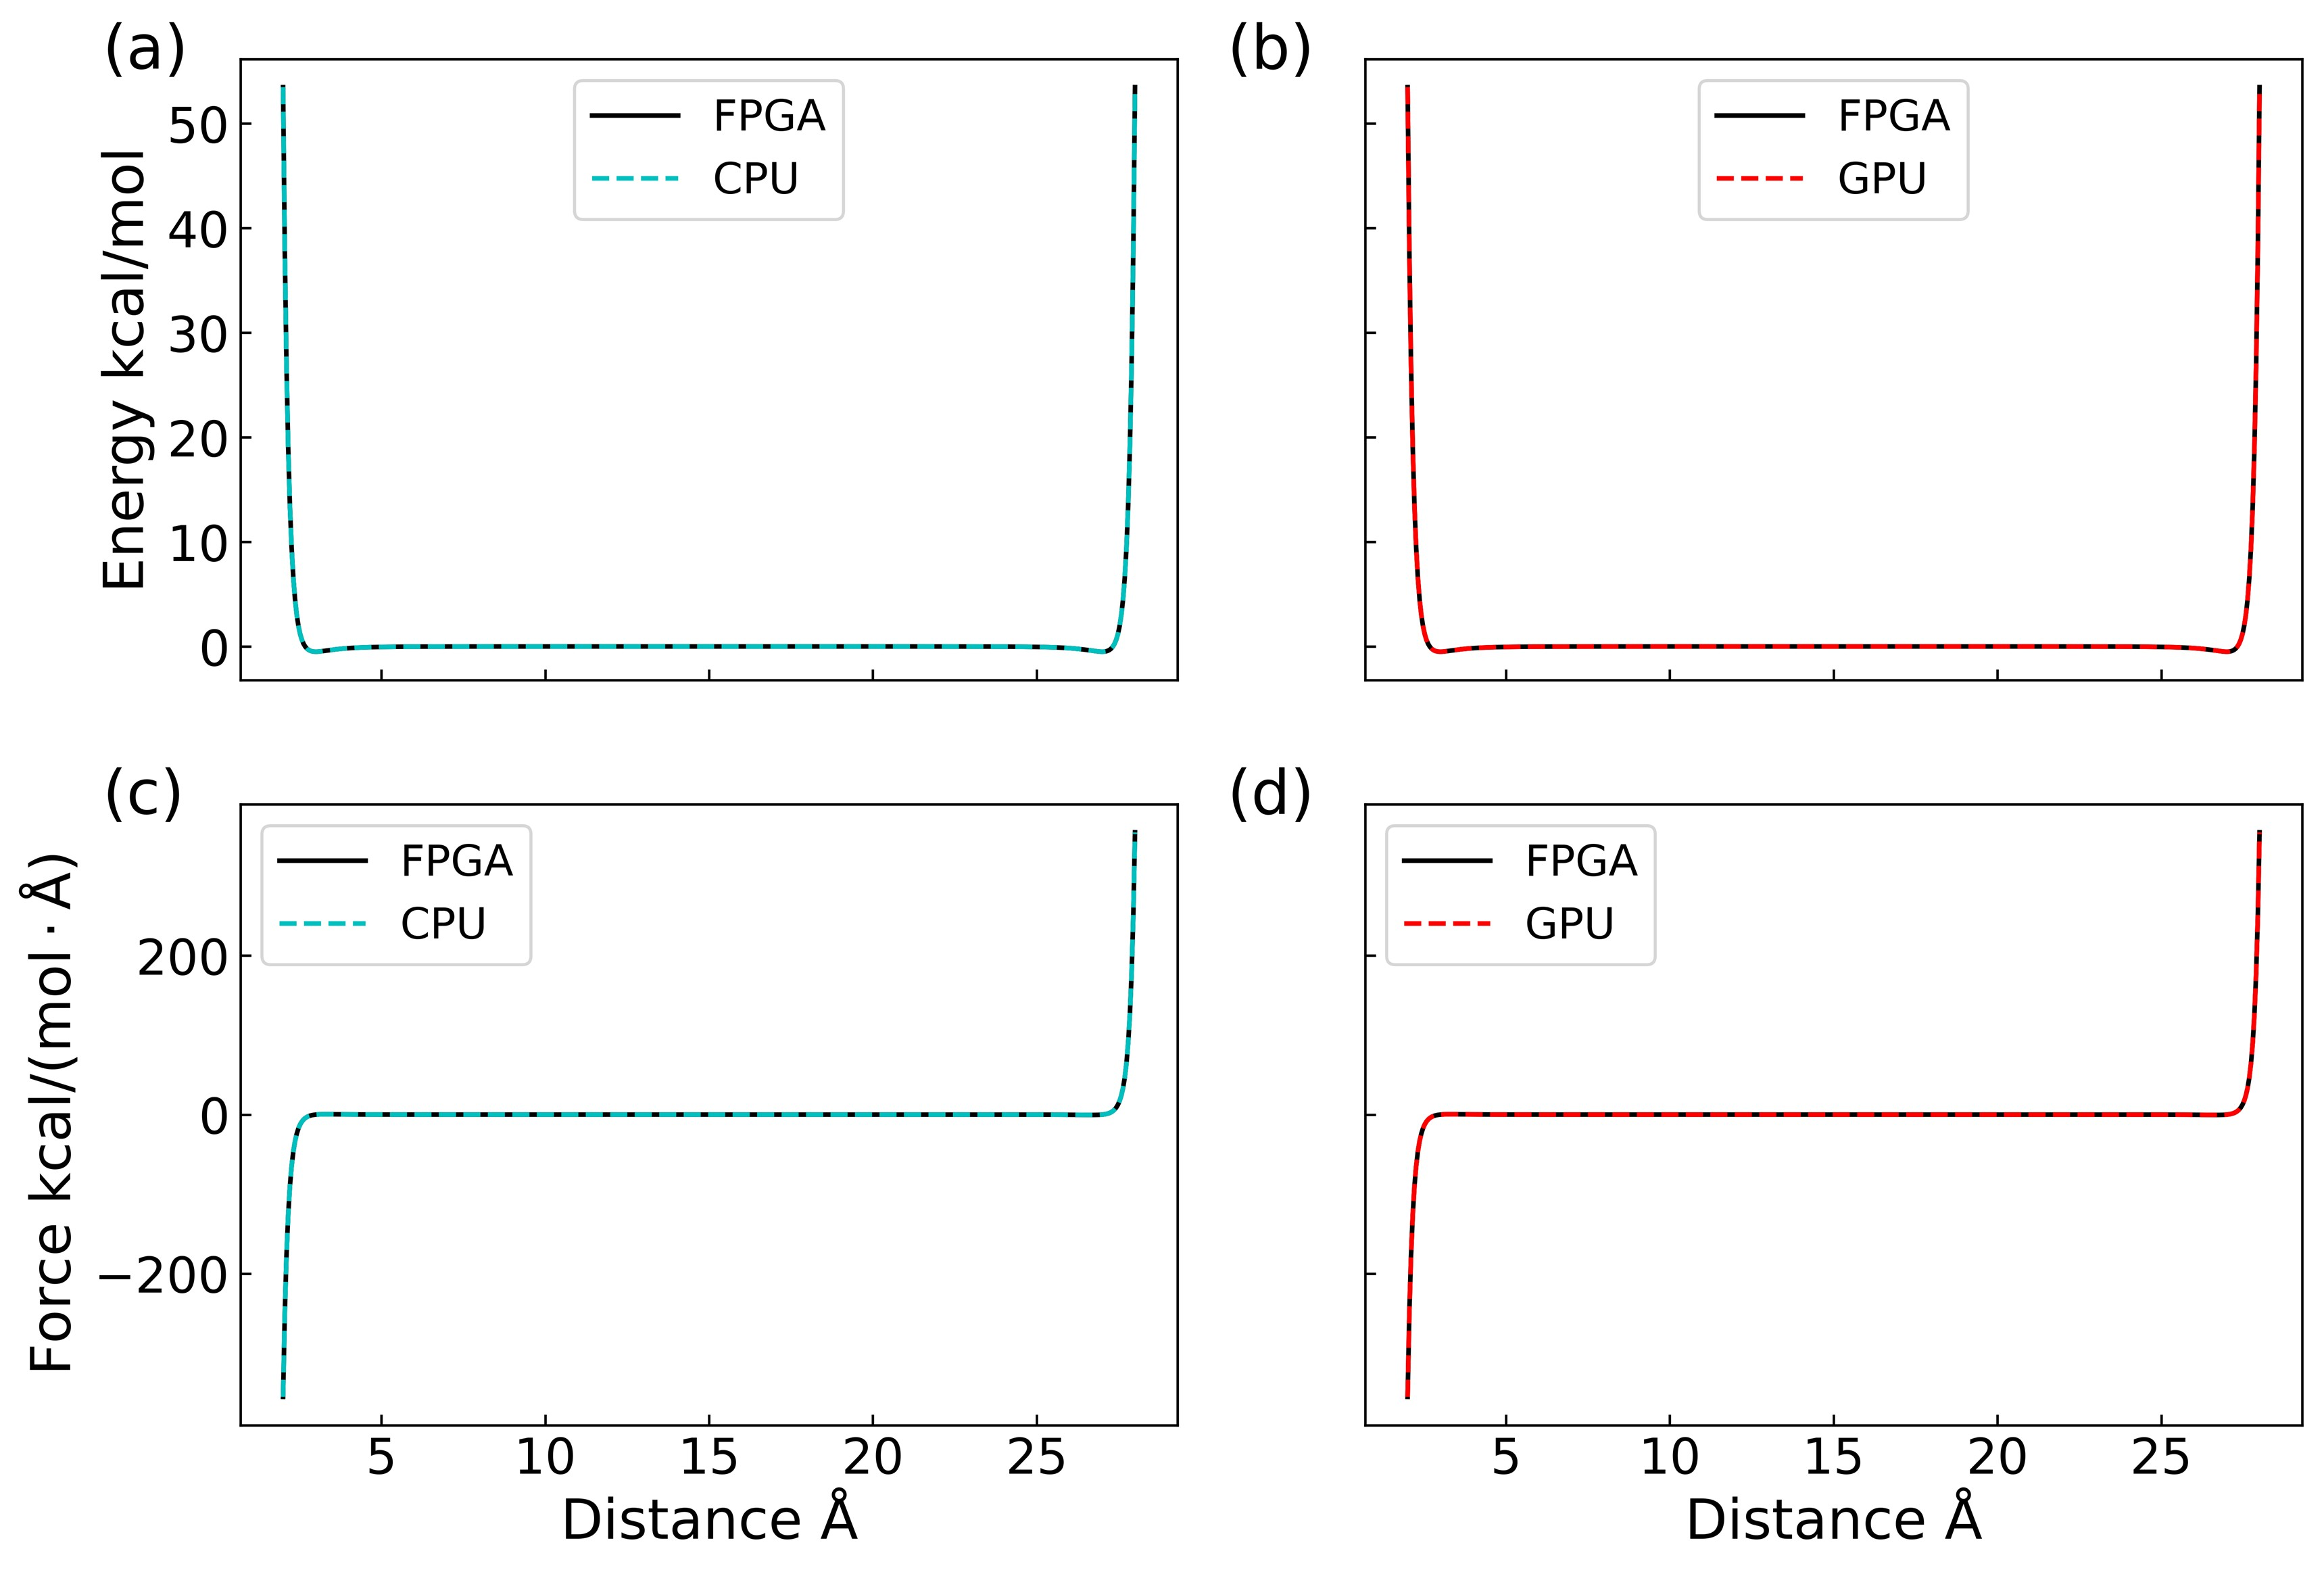
\includegraphics[angle=0, width=1.0\textwidth]{figures/lj_energy_force.jpg}
	\caption[Comparison of energy and single-particle forces vs. inter-particle distance in 30~\AA\ periodic box]{Comparison of two-particle LJ system energy and single-particle forces as functions of inter-particle distance in 30~\AA\ periodic box: (a) Total energy comparison between FPGA and CPU calculations. (b) Total energy comparison between FPGA and GPU calculations. (c) Single-particle force comparison between FPGA and CPU calculations. (d) Single-particle force comparison between FPGA and GPU calculations.}
	\label{lj_energy_force}
\end{figure*}

\begin{figure*}[!ht]
	\centering
	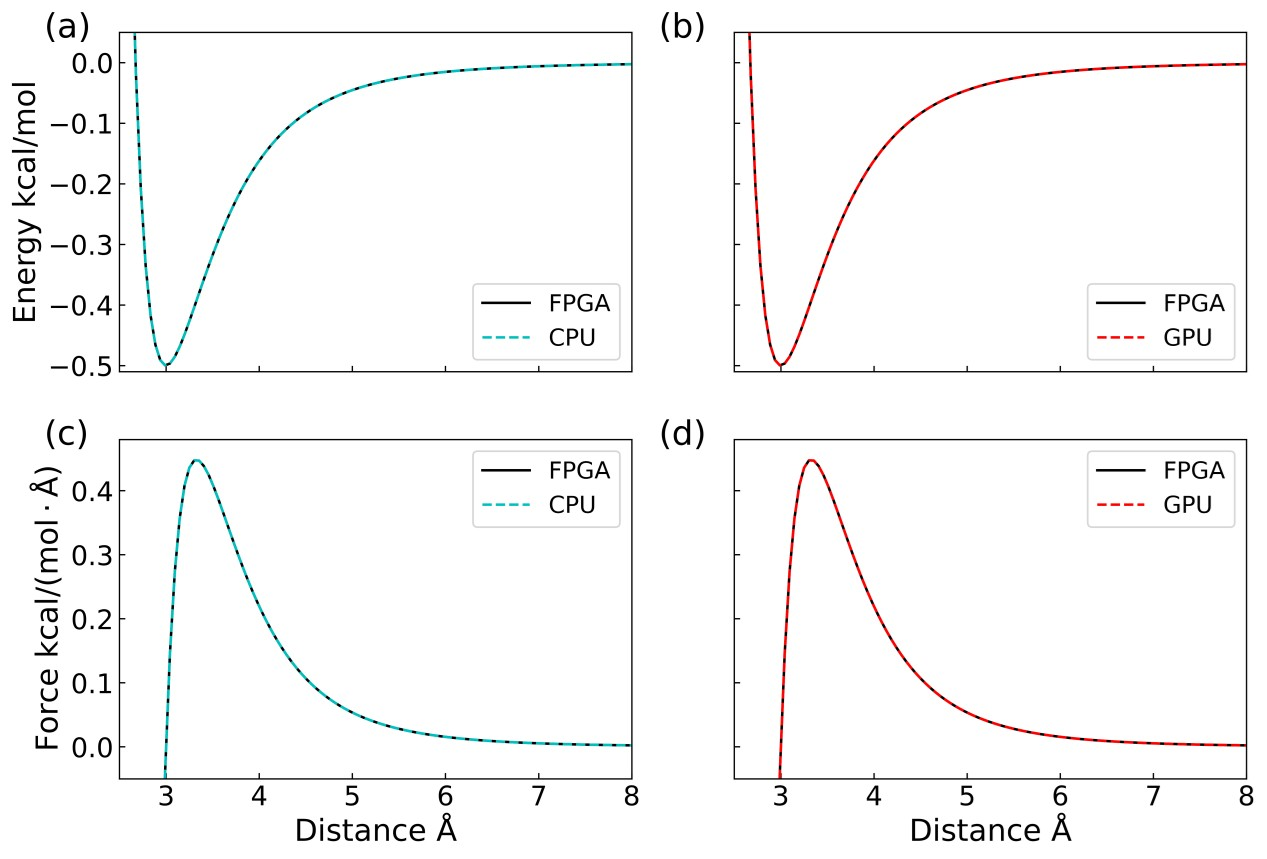
\includegraphics[angle=0, width=1.0\textwidth]{figures/zoom_lj_energy_force.jpg}
	\caption[Zoom-in comparison of energy and forces (2.5--8~\AA) in 30~\AA\ periodic box]{Detailed comparison of two-particle LJ system energy and single-particle forces from 2.5~\AA\ to 8~\AA\ in 30~\AA\ periodic box: (a) Total energy comparison (FPGA vs. CPU). (b) Total energy comparison (FPGA vs. GPU). (c) Single-particle force comparison (FPGA vs. CPU). (d) Single-particle force comparison (FPGA vs. GPU).}
	\label{zoom_lj_energy_force}
\end{figure*}


Building upon successful validation of the Lennard-Jones (LJ) potential in two-particle systems, this work extends characterization to a 15-atom Argon cluster under periodic boundary conditions (30 \AA cubic box). Parameters derived from the CHARMM force field ($\sigma$ = 3.8220 \AA, $\varepsilon$ = 0.238065 kcal/mol) were implemented with a 12 \AA~non-bonded interaction cutoff. Five distinct structural configurations were tested across FPGA, GPU, and CPU platforms using identical hardware setups as previously reported.
The LJ potential energy calculations (Table~\ref{tbl:argon}) demonstrate <5\% inter-platform RMS deviation across all test cases, confirming FPGA implementation accuracy. This cross-platform consistency validates the FPGA's computational precision in handling LJ interactions through optimized parallel architectures and memory bandwidth utilization.
\begin{table}[!ht]
	\centering
	\begin{tabular}{cccc}
		\hline
		\multicolumn{1}{l}{} & \multicolumn{3}{c}{Potential Energy (kJ/mol)} \\ \cline{2 - 4}
		& FPGA      & CPU       & GPU       \\ \hline
		Frame1               & 0.923459  & 0.922628  & 0.922628  \\
		Frame2               & -2.184186 & -2.182222 & -2.182222 \\
		Frame3               & -3.207323 & -3.204440 & -3.204439 \\
		Frame4               & -1.750265 & -1.748692 & -1.748693 \\
		Frame5               & -1.624073 & -1.622612 & -1.622612 \\ \hline
	\end{tabular}
	\caption[Inert gas in test results]{Total LJ interaction energy calculated for a system of fifteen argon atoms on five structures.}
	\label{tbl:argon}
\end{table}


After validating the energy calculations of the protein system, we further conducted MD simulations on the FPGA platform to verify its capability for authentic simulation tasks. As illustrated in Figures 5-15 and 5-16, the test system employed the dihydrofolate reductase (DHFR) model, a benchmark protein consisting of 159 amino acid residues and 2489 atoms commonly used in computational studies. The FPGA accelerator utilized the Xilinx Virtex UltraScale+ VU37P chip for implementation.

The simulation parameters included a time step of 2 fs and 3D-FFT with two spatial resolutions: 32×32×32 and 64×64×64. Comparative analyses were performed against CPU and GPU implementations. During the 3D-FT process, systematic errors were observed, primarily attributed to two factors: (1) The FPGA's native FFT IP core only supports matrix dimensions as powers of two (e.g., 32-bit or 64-bit inputs), and (2) The FFT v9.0 IP core offers both 32-bit floating-point and fixed-point modes, with distinct resource consumption trade-offs.


 \begin{figure}[H]
	\centering
	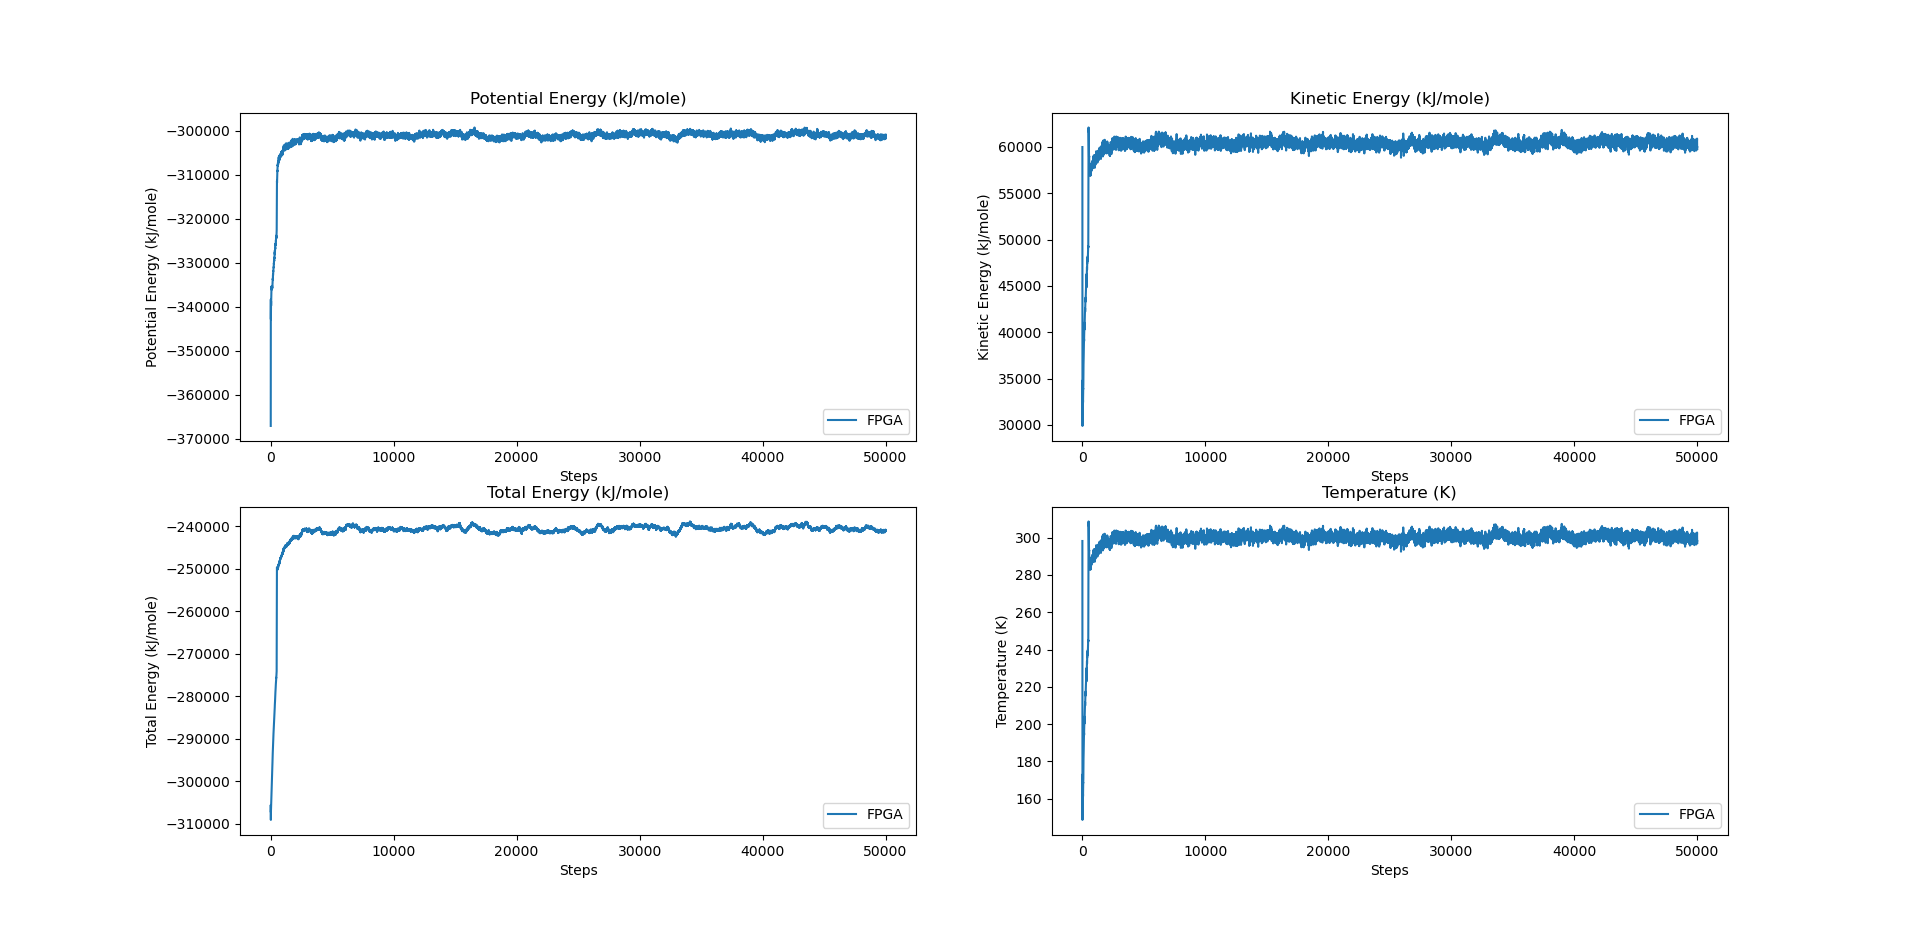
\includegraphics[angle=0,width=1.0\textwidth]{./figures/Fig12_fpga_fft_64.png}
	\caption{18,000 Argon  gas particles, using Inspur FPGA accelerator card plus OpenMM software interface for calculation results, data energy calculation results. (a) is the overall Energy Waveform.}
\end{figure}

 \begin{figure}[H]
	\centering
	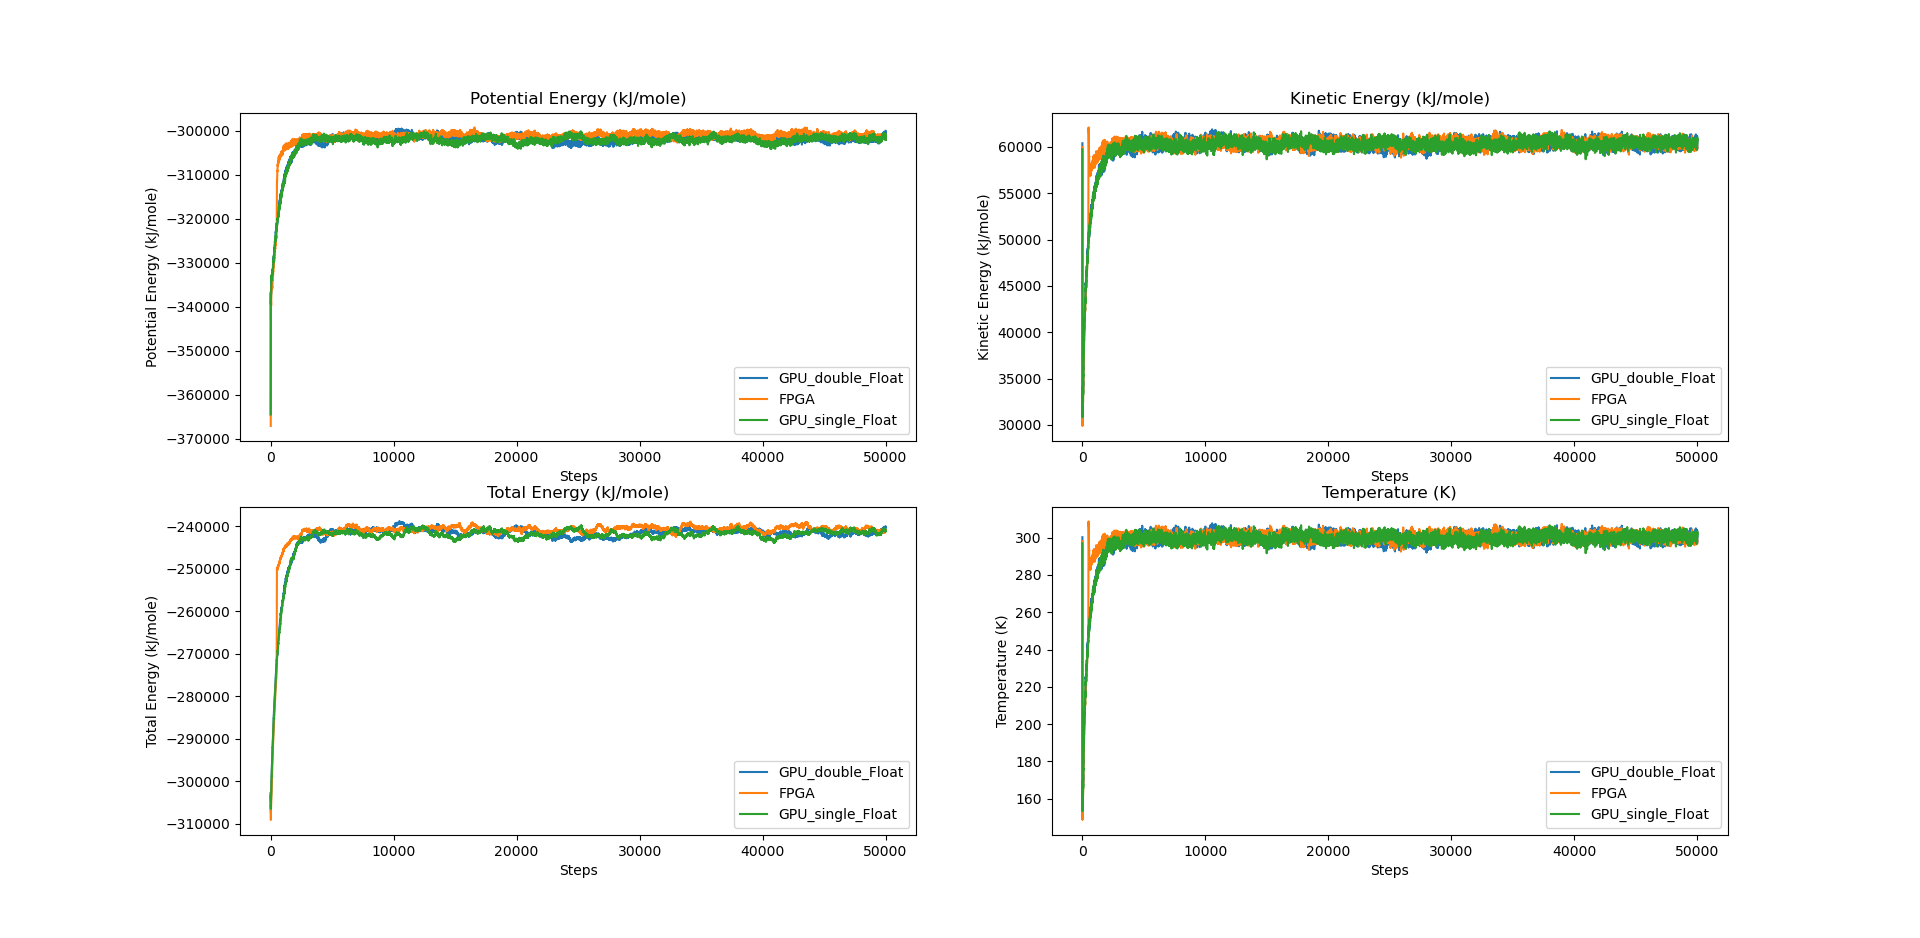
\includegraphics[angle=0,width=1.0\textwidth]{./figures/fpga_fft_32.png}
	\caption{DHFR protein system simulation results, PME algorithm using 32 point three-dimensional FFT transformation. Compared with the FPGA accelerated version, CPU and GPU versions, the data calculation results are basically the same.}
\end{figure}

% computational details of Argon and DHFR
% and the results

\section{Discussion}

The Inspur F37X FPGA accelerator card was selected for its advanced programmable logic architecture, offering high flexibility and precise customization to address specific algorithmic requirements of the project. This adaptability effectively overcomes performance bottlenecks inherent in traditional computing architectures, enabling breakthroughs in technical barriers and fostering innovative research pathways. The accelerator card leverages the Xilinx Virtex UltraScale+ VU37P chip, integrating 8GB HBM2 high-bandwidth memory with a bandwidth of 460GB/s, delivering 28.1 TOPS INT8 compute performance at <75W power consumption. This configuration enables high-speed AI inference and scientific computing while maintaining energy efficiency, outperforming CPUs in scenarios requiring low latency and high throughput .

Performance comparisons with mainstream GPUs (e.g., NVIDIA GTX 1650) revealed that the FPGA platform currently matches the Intel i5-8400 CPU in efficiency but lags behind GPUs. This gap stems from incomplete optimization of the FPGA implementation and suboptimal resource utilization. For instance, the Virtex UltraScale+ architecture's DSP slices and logic units require further pipeline optimization and operator fusion to fully exploit parallelism. Despite this, the FPGA demonstrates strong accuracy in energy calculations across MD simulations. For example, the Root Mean Square Error (RMSE) between FPGA and CPU/GPU energy computations for Lennard-Jones (LJ) interactions is $3.5 times 10^{-6}$ kcal/mol, validating computational consistency. Multi-particle argon system tests further confirmed negligible energy deviations, while CHARMM TIP3P water model simulations validated the fidelity of LJ and electrostatic interactions under rigid constraints and Particle Mesh Ewald (PME) treatments .

The choice of FP32 floating-point arithmetic in HLS-based three-level interpolation modules prioritizes precision over immediate resource savings. FP32's 24-bit mantissa ensures minimal cumulative errors in intermediate calculations, critical for algorithms like interpolation where decimal precision impacts convergence. While lower-precision types (FP16/INT8) might suffice for some tasks, they risk instability in complex workflows requiring high dynamic range. This approach aligns with future FPGA advancements, where increased logic resources will enable seamless integration of FP32-optimized IP blocks without sacrificing accuracy .

In contrast to RTL designs, which demand meticulous state machine engineering and timing constraint programming (3-5$\times$ longer development cycles), HLS accelerates prototyping through high-level abstractions. Tools like Vivado HLS automate resource allocation and pipeline optimization, reducing manual intervention. However, RTL remains essential for ultra-optimized, latency-sensitive modules, such as those requiring strict deterministic timing—a balance critical for MD applications where both speed and precision are paramount .
\section{Conclusions}

\noindent
In MD hardware design, the finite-range interaction force is one of the modules that can best reflect the parallelism of the hardware, this design adopts the classical acceleration algorithms such as the proximity list lookup method, and synthesizes the performance of each expansion module of the FPGA device to make a reasonable design of the module. 
In the process of particle-pair interaction force calculation, a large amount of intermediate computational data will be generated, which need to be reasonably spliced and cached, relying only on chip memory is far from enough.\\

\noindent
In this chapter, the basic definition, main characteristics and development history of FPGA are summarized, and compared and analyzed with general-purpose processors. 
An all-hardware module is designed to accelerate the calculation of MD, which is aimed at increasing the calculation speed, and the pipeline technique is used to optimize the allocation of tasks in the whole parallel system. 
The Single Instruction Multiple Data Stream (SIMD) approach is utilized to significantly improve the computational efficiency. At the same time, we have built a software framework dedicated to this scheme, which can be used to accelerate the data processing of the circuit.\\

\noindent
To better exploit its parallel potential, we comprehensively compare existing high-speed interfaces and memory devices, and comparatively analyze existing high-speed architectural designs.
The new generation of high-bandwidth memories, such as HBM2 memories, are used to fully compare the impact of existing memory structures on computational performance in MD design.
A lot of work has been done using DDR4 high-speed interface, and the computation uses polling algorithm to improve the access efficiency.
The new generation of high-speed and high-bandwidth multi-parallel interface HBM memory is adopted, so that the read and write access to external mass storage can be completed while the parallel computation of multi-path data. 
The optimized design of the underlying RTL circuits fundamentally improves the efficiency of data read and write registers, and more than doubles the efficiency of reading and writing external storage. Therefore, the rational use of external mass memory devices is fully considered in the design process. 
We selected the same cloud platform Xilinx UV9P/UV37P chip, in the design of the DDR4 and HBM2 two relatively efficient memory, because in the MD calculation there are a large number of intermediate computational data, which write data directly related to the particle information, so the storage of data need to be stored in an independent storage interval, the DDR is a single read-write channel, the HBM support for 32 independent read-write channels, which for the Particle computing read/write storage space greatly improves the data throughput efficiency.
The use of multi-channel computation improves the efficiency of particle reading and writing to external memory, but the consumption of on-chip resources by the read/write driver needs to be fully considered. We adopt the progress proofreading module to supervise the multi-channel data to ensure the orderly reading and writing of data.\\

\noindent
For the same MD simulation system, the data are "sliced" by matching the computational nodes and sent to the designated computational unit.
The computation unit needs to adopt a reasonable floating-point computation mode. In this design, we compare a variety of numerical computation models, using multi-order linear interpolation, respectively, for the first-order, second-order, third-order computation models, each section of the fitted curve to do a reasonable cut modeling, such as the above $X ^ {-7} $, to build the numerical interpolation table. 
The interpolation table is transferred to the on-chip memory via high-speed AXI lite protocol, which ensures high computational efficiency. 
At the same time, HLS advanced compilation means and RTL design means are used, and finally RTL design circuits are used to ensure computational efficiency. 
The interpolation algorithms are compared with Newtonian interpolation, Hamiltonian interpolation and Legendre interpolation.\\

\noindent
After the same MD simulation system has been divided into chunks, it is necessary to design a reasonable proximity force computation supervision module, which needs to record the computational progress of each module data. 
Assuming that a simulation system is divided into 1000 or more sub-Cells, and at the same time, the means of separate computation in the upper and lower hemispheres are used, which undoubtedly increases the difficulty of designing the supervision module. 
We adopt a multi-level supervision means to ensure that the computation is carried out efficiently.\\


\clearpage
%
% Reference
%

\bibliographystyle{unsrt}
\bibliography{main}


\end{document}